%% chapter09_slides.tex
%% Chapter 9: Population Methods
%% Algorithms for Optimization, 2nd ed. (2026) --- Kochenderfer & Wheeler
%% Compile: pdflatex -interaction=nonstopmode chapter09_slides.tex  (run twice)

\documentclass[aspectratio=169,10pt]{beamer}

\usetheme{Madrid}
\usecolortheme{seahorse}
\setbeamertemplate{footline}[frame number]
\setbeamertemplate{navigation symbols}{}

%% Packages
\usepackage{amsmath,amssymb,mathtools}
\usepackage{graphicx}
\usepackage{listings}
\usepackage{xcolor}
\usepackage{booktabs}
\usepackage{tikz}
\usepackage{algorithm}
\usepackage{algpseudocode}
\usepackage{microtype}
\usepackage{multicol}

\graphicspath{{figures/}}

%% Python listings style
\lstdefinestyle{python}{
  language=Python,
  basicstyle=\ttfamily\scriptsize,
  keywordstyle=\color{blue!80!black}\bfseries,
  commentstyle=\color{green!50!black}\itshape,
  stringstyle=\color{orange!80!black},
  numbers=left,
  numberstyle=\tiny\color{gray},
  stepnumber=1,
  numbersep=4pt,
  frame=single,
  backgroundcolor=\color{gray!7},
  breaklines=true,
  showstringspaces=false,
  tabsize=4,
  captionpos=b,
}

%% Maths shortcuts
\newcommand{\bx}{\mathbf{x}}
\newcommand{\bv}{\mathbf{v}}
\newcommand{\ba}{\mathbf{a}}
\newcommand{\bb}{\mathbf{b}}
\newcommand{\bc}{\mathbf{c}}
\newcommand{\R}{\mathbb{R}}
\newcommand{\norm}[1]{\left\|#1\right\|}

%% Title info
\title[Ch.\ 9: Population Methods]{Chapter 9: Population Methods}
\subtitle{Algorithms for Optimization, 2nd Edition (2026)}
\author{Kochenderfer \& Wheeler}
\institute{Adapted for Lecture Slides}
\date{2026}

% ---------------------------------------------------------------
\begin{document}
% ---------------------------------------------------------------

\begin{frame}
  \titlepage
\end{frame}

% ---------------------------------------------------------------
\begin{frame}{Chapter Outline}
  \tableofcontents
\end{frame}

% ---------------------------------------------------------------
\section{Population Iteration}
% ---------------------------------------------------------------

\begin{frame}[allowframebreaks]{Motivation: Why Use a Population of Solutions?}

  All the optimization methods covered in previous chapters share one
  structural feature: they maintain a \emph{single} candidate design
  point $\bx$ and iteratively improve it.  This single-point strategy
  works well for smooth, unimodal objectives --- that is, functions with
  exactly one minimum and no misleading valleys --- but it has a
  fundamental weakness: once the search converges to a local minimum,
  there is no information anywhere else in the design space to draw on,
  and the algorithm simply stops improving.

  \textbf{Population methods} take a fundamentally different approach.
  Instead of tracking one design, they maintain a \emph{collection}
  (a ``population'') of $m$ (m) candidate solutions
  $\bx^{(1)}, \bx^{(2)}, \ldots, \bx^{(m)}$ and evolve all of them
  simultaneously through many iterations called \emph{generations}.
  Here, $\bx^{(i)}$ (x superscript i in round brackets) denotes the
  $i$-th (i-th) \emph{individual} in the population, and the superscript
  in round brackets distinguishes it from an exponent.

  \begin{columns}[T]
    \begin{column}{0.55\textwidth}
      \begin{block}{Four Key Advantages of Population Methods}
        \textbf{1. Information sharing across the design space.}
        Because different individuals occupy different regions of the
        design space simultaneously, the algorithm can detect structure
        such as ridges, valleys, and flat plateaus that a single-point
        method exploring sequentially would never observe.  Individuals
        from different regions can exchange useful structural information
        through crossover or attraction mechanisms.

        \textbf{2. Better ability to escape local minima.}
        A single individual trapped near a poor local minimum may never
        escape if the surroundings provide no downhill direction.  In
        a population, however, an individual from a completely different
        region --- one that happens to be near the global optimum ---
        can provide ``genetic material'' (via crossover, velocity
        attraction, or similar mechanisms) that rescues the stuck
        individuals.

        \textbf{3. Natural parallelism.}
        All $m$ (m) objective function evaluations in a single
        generation are completely independent of one another.  They
        can therefore be computed simultaneously on a multi-core
        processor or distributed across a cluster, making population
        methods particularly well-suited to modern hardware.

        \textbf{4. Diversity supports global exploration.}
        A population that is spread broadly across the design space is
        much more likely to have at least one individual in the
        basin of attraction of the global minimum, compared to a
        single starting point chosen at random.  This is especially
        important when the design space is high-dimensional.
      \end{block}
    \end{column}
    \begin{column}{0.43\textwidth}
      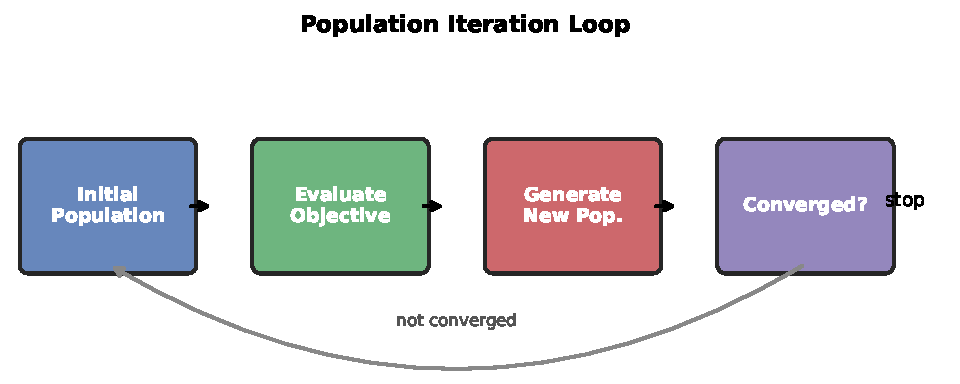
\includegraphics[width=\linewidth]{fig_population_iteration.pdf}
      \vspace{4pt}
      \footnotesize
      The fundamental population loop: initialise $m$ individuals,
      evaluate the objective $f$ at each, generate a new population
      using a method-specific rule, and check for convergence.  This
      loop structure is shared by all methods in this chapter --- the
      only difference between methods is how the new population is
      generated from the current one.
    \end{column}
  \end{columns}

  \begin{alertblock}{Key Insight: Diversity versus Convergence}
    Every population method faces a fundamental tension between
    \emph{exploration} (keeping individuals spread across the design
    space to avoid missing the global optimum) and \emph{exploitation}
    (concentrating individuals near the current best solutions to refine
    them efficiently).  Too much exploration wastes evaluations on
    unproductive regions; too much exploitation leads to premature
    convergence at a local minimum.  The methods in this chapter each
    resolve this tension in a different way, and understanding that
    trade-off is the key to choosing the right method for a given problem.
  \end{alertblock}

\end{frame}

% ---------------------------------------------------------------
\begin{frame}[allowframebreaks]{Population Iteration: The General Template}

  Before studying specific algorithms (genetic algorithms,
  differential evolution, particle swarm optimization, etc.), it is
  helpful to see that they all share the same high-level algorithmic
  skeleton.  Understanding this shared structure makes it easy to
  switch between methods: only one step changes.

  \begin{block}{General Population Method --- Algorithm 9.1}
    \begin{enumerate}
      \item \textbf{Initialise} the population
            $\mathcal{P} = \{\bx^{(1)}, \ldots, \bx^{(m)}\}$, typically
            by drawing each individual uniformly at random from the
            feasible design space (the set of all allowed design vectors).
            This ensures no region of the space is systematically
            excluded from the initial search.
      \item For $k = 1, 2, \ldots, k_{\max}$ (k sub max, the maximum
            number of generations, a user-specified budget):
        \begin{enumerate}[(a)]
          \item Evaluate $f(\bx^{(i)})$ for every individual $i$ in the
                current population, where $f$ is the objective function
                we are trying to minimise.
          \item \textbf{Generate} a new population using a
                method-specific rule.  This rule typically rewards
                lower-objective individuals (selection), combines
                information from multiple parents (crossover or
                attraction), and introduces randomness (mutation or
                random walks).  \emph{This is the only step that
                differs between methods.}
        \end{enumerate}
      \item Return the best individual found across all generations:
            $\bx^{*} = \arg\min_{i} f(\bx^{(i)})$, where $\arg\min$
            (``argmin'', meaning ``the argument that minimises'')
            extracts the individual with the smallest objective value.
    \end{enumerate}
  \end{block}

  Here $k_{\max}$ (k sub max) is typically set by specifying a total
  function evaluation budget.  Since each generation performs $m$ (m)
  evaluations (one per individual), the total number of evaluations
  is $m \times k_{\max}$.

  \begin{exampleblock}{Worked Example: Counting Evaluations}
    Suppose we run a population method with $m = 50$ individuals
    and $k_{\max} = 100$ generations.  The total number of objective
    function evaluations is $50 \times 100 = 5{,}000$.  If each
    evaluation takes 0.1 seconds, the total wall-clock time is
    $5{,}000 \times 0.1 = 500$ seconds $\approx 8.3$ minutes.
    If the evaluations can be parallelised across 50 CPU cores,
    the time reduces to $100 \times 0.1 = 10$ seconds --- a
    50-fold speed-up.  This illustrates why population methods
    are so attractive for computationally expensive objectives.
  \end{exampleblock}

  \begin{alertblock}{Key Insight: One Skeleton, Many Algorithms}
    The only part that differs between genetic algorithms, differential
    evolution, PSO, and other methods in this chapter is \emph{step
    2(b)}: how the new population is generated from the current one.
    The initialisation and termination logic are identical.  When you
    encounter a new population method, your first task should be to
    identify exactly what rule it uses in step 2(b).
  \end{alertblock}

\end{frame}

\begin{frame}[fragile]{Population Iteration: Python Skeleton}
\begin{lstlisting}[style=python, caption={Generic population method skeleton (Python / NumPy)}]
import numpy as np

def population_method(f, bounds, pop_size=50, k_max=100, rng=None):
    """Generic population loop.  Override `step` to specialise."""
    rng = rng or np.random.default_rng()
    lo, hi = np.array(bounds).T          # lower and upper bounds per dimension
    # Step 1: uniform initialisation across the feasible space
    population = rng.uniform(lo, hi, (pop_size, len(lo)))
    for _ in range(k_max):
        # Step 2a: evaluate objective at every individual
        y = np.array([f(x) for x in population])
        # Step 2b: method-specific update (returns new population of same size)
        population = step(population, y, rng)
    # Return best individual found
    y = np.array([f(x) for x in population])
    return population[np.argmin(y)]
\end{lstlisting}

  In this skeleton, \texttt{bounds} is a list of \texttt{(lo, hi)}
  pairs, one per design variable dimension.  For example, if the
  design space is the square $[-3, 3]^2$, then
  \texttt{bounds = [(-3, 3), (-3, 3)]}.  The array
  \texttt{population} has shape \texttt{(pop\_size, n)}, where
  \texttt{pop\_size} is $m$ (m) and \texttt{n} is the number of
  design variables.  The function \texttt{step} --- which you
  override when implementing a specific method --- takes the current
  population matrix and its objective values and returns a new
  population matrix of the same shape.  To implement a GA, you
  replace \texttt{step} with selection + crossover + mutation; for
  DE, you replace it with the DE mutation rule; for PSO, with the
  velocity-position update.  Everything else stays the same.

\end{frame}

% ---------------------------------------------------------------
\section{Genetic Algorithms}
% ---------------------------------------------------------------

\begin{frame}[allowframebreaks]{Genetic Algorithms: Biological Inspiration and Overview}

  Genetic Algorithms (GAs) are the oldest and most well-known class
  of population methods.  They were developed by John Holland in the
  1970s and draw their inspiration from Darwinian natural selection:
  individuals that are better adapted to their environment survive
  and reproduce more often, gradually shifting the population toward
  higher fitness over many generations.

  In the optimization context, ``fitness'' corresponds to having a
  low objective value $f(\bx)$ (since we are minimising, a lower
  objective is ``better'' just as a better-adapted organism survives
  more easily).  Each individual $\bx$ is called a
  \emph{chromosome}, and each component $x_j$ (x sub j) of the
  design vector is called a \emph{gene}.  Genes may be real-valued
  (for continuous design spaces) or binary (for combinatorial problems).

  \begin{columns}[T]
    \begin{column}{0.58\textwidth}
      \begin{block}{Three Core Operators --- Algorithm 9.2}
        A GA applies three operators each generation in sequence:
        \begin{enumerate}
          \item \textbf{Selection} --- decide which individuals get to
                ``reproduce'' (become parents of the next generation),
                favouring those with lower objective values so that
                useful gene combinations are propagated forward.
          \item \textbf{Crossover} (also called \emph{recombination})
                --- combine the chromosomes (design vectors) of two
                selected parent individuals to create offspring.  This
                is the mechanism by which good gene combinations
                discovered in different parts of the population can
                be merged into a single offspring.
          \item \textbf{Mutation} --- randomly perturb individual
                genes of the offspring with a small probability.
                This ensures new gene values can appear that were
                not present in any parent, preventing the population
                from being permanently limited to gene combinations
                seen in the initial generation.
        \end{enumerate}
      \end{block}

      \medskip
      Before selection can choose parents, we must convert objective
      values (where lower is better) into \emph{fitness} values
      (where higher is better).  The standard transformation is:
      \[
        \text{fitness}_i
        = \max\bigl\{f(\bx^{(1)}), \ldots, f(\bx^{(m)})\bigr\}
          - f(\bx^{(i)})
      \]
    \end{column}
    \begin{column}{0.40\textwidth}
      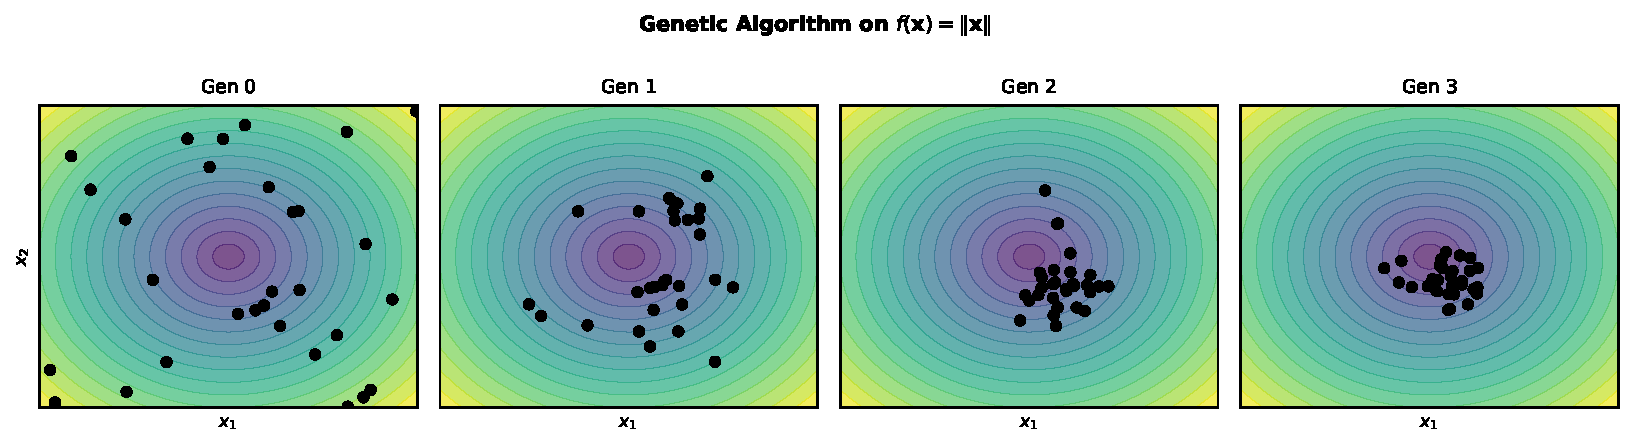
\includegraphics[width=\linewidth]{fig_ga_evolution.pdf}
      \footnotesize
      Four successive generations of a genetic algorithm minimising
      $f(\bx) = \|\bx\|$ (the Euclidean distance from the origin,
      i.e., $\sqrt{x_1^2 + x_2^2}$, whose minimum is 0 at the
      origin).  The population visibly concentrates toward $\bx =
      \mathbf{0}$ (the global minimum) as generations pass.
    \end{column}
  \end{columns}

  \begin{block}{Notation: The Fitness Conversion Formula}
    In the formula above:
    \begin{itemize}
      \item $\max\{f(\bx^{(1)}), \ldots, f(\bx^{(m)})\}$ is the
            largest (worst) objective value among all $m$ (m)
            individuals in the current population.
      \item $f(\bx^{(i)})$ is the objective value of individual $i$.
      \item $\text{fitness}_i$ (fitness sub i) is the resulting
            fitness score for individual $i$.
    \end{itemize}
    Subtracting the individual's objective from the maximum gives
    a non-negative number: the worst individual (with the highest
    objective) gets fitness $= 0$, while the best individual
    (with the lowest objective) gets the highest fitness value.
    All other individuals lie in between.
  \end{block}

  \begin{alertblock}{How to Read This Formula}
    Think of it this way: if the worst objective in the population
    is 10 and an individual has objective 3, its fitness is
    $10 - 3 = 7$.  Another individual with objective 9 gets
    fitness $10 - 9 = 1$.  The individual with fitness 7 is
    seven times more attractive to roulette-wheel selection than
    the individual with fitness 1.  As the population improves
    over generations, the maximum objective shrinks, and so do
    the fitness values --- a natural self-calibration that keeps
    selection pressure stable.
  \end{alertblock}

\end{frame}

% ------- 9.2.1 Selection -------
\begin{frame}[allowframebreaks]{9.2.1 Selection: Choosing Which Individuals Reproduce}

  Selection is the mechanism by which a genetic algorithm applies
  ``survival of the fittest''.  The goal is to choose parent
  individuals for the next generation so that individuals with lower
  objective values (higher fitness) are more likely to pass their
  genes on, while still allowing some less-fit individuals a chance
  to reproduce (to preserve diversity).  Three common selection
  methods are described below.

  \begin{columns}[T]
    \begin{column}{0.56\textwidth}
      \begin{block}{Method 1: Truncation Selection}
        Keep only the $k$ (k, the truncation size) best individuals
        --- those with the $k$ lowest objective values --- and discard
        all others.  New parent pairs are sampled uniformly at random
        from this elite subset of size $k$.  Conceptually: sort the
        population by objective value, take the top $k$, and sample
        from those.  The parameter $k$ is typically set to around
        $10\%$ to $20\%$ of the population size (for example,
        $k = 10$ out of $m = 100$).

        The trade-off is that truncation can rapidly reduce genetic
        diversity, since only $k$ unique parent chromosomes are
        available.  If $k$ is too small, the population can
        prematurely collapse to a single local minimum.
      \end{block}

      \begin{block}{Method 2: Tournament Selection}
        To choose each parent, draw $k$ (k, the tournament size)
        individuals at random from the full population (without
        replacement) and select the one with the best (lowest)
        objective value among those $k$ competitors.  The
        ``tournament size'' $k$ controls selection pressure:
        \begin{itemize}
          \item $k = 1$: no pressure --- all individuals are equally
                likely to be selected regardless of quality.
          \item $k = 2$: mild pressure --- two individuals compete
                and the better one wins.
          \item $k = m$: maximum pressure --- only the globally best
                individual is ever selected.
        \end{itemize}
        Tournament selection is widely used because it is efficient,
        requires no global fitness sum, and lets you dial pressure
        via a single integer $k$.
      \end{block}

      \begin{block}{Method 3: Roulette-Wheel (Fitness-Proportional) Selection}
        Assign each individual $i$ a selection probability proportional
        to its fitness:
        \[
          P(\text{select individual } i)
          = \frac{\text{fitness}_i}{\displaystyle\sum_{j=1}^{m} \text{fitness}_j}
        \]
        Here $\sum_{j=1}^{m}$ (Sigma from $j$ equals 1 to $m$,
        meaning ``sum over all $m$ individuals in the population'')
        ensures all probabilities add to 1, forming a valid
        probability distribution.

        The worst individual always has fitness $= 0$, so
        $P(\text{select worst}) = 0$: it can never be selected.
        The best individual has the largest probability of selection.
      \end{block}
    \end{column}
    \begin{column}{0.42\textwidth}
      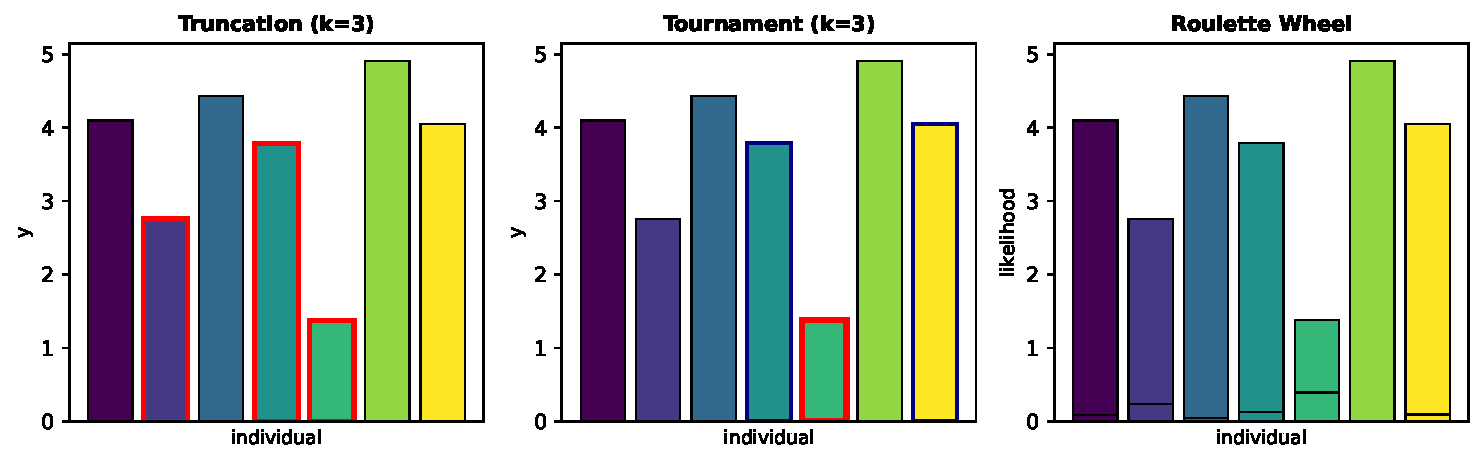
\includegraphics[width=\linewidth]{fig_selection_methods.pdf}
      \footnotesize
      \textbf{Left}: Truncation selection --- the three individuals
      with highlighted borders are the top-$k$ elite; only these
      are used as parents for the next generation.
      \textbf{Centre}: Tournament selection --- a random subset of
      individuals competes and the winner (lowest objective) becomes
      a parent.
      \textbf{Right}: Roulette wheel --- each bar height represents
      the selection probability of one individual, proportional to
      its fitness.
    \end{column}
  \end{columns}

  \begin{alertblock}{How to Read the Roulette-Wheel Formula}
    Imagine drawing a roulette wheel where each individual $i$ gets
    a slice of the wheel whose width is proportional to its fitness
    score.  Spinning the wheel and seeing where it lands is
    equivalent to sampling from the probability distribution
    $P(\text{select } i) \propto \text{fitness}_i$.  An individual
    with twice the fitness of another gets twice as wide a slice and
    is twice as likely to be selected.  This is the most
    ``theoretically natural'' formulation of selection pressure, but
    it can be unstable when one individual is far fitter than all
    others: it then dominates the wheel and the effective population
    reduces to a single individual.  Tournament selection avoids
    this instability.
  \end{alertblock}

  \begin{alertblock}{Practical Guidance: Which Method to Choose?}
    Truncation is simple and fast but can reduce diversity; it works
    well when the objective landscape is relatively smooth with few
    local minima.  Tournament selection is the most flexible: setting
    $k = 2$ or $k = 3$ is a common default that provides moderate
    selection pressure.  Roulette wheel is theoretically elegant but
    sensitive to scale; it is less commonly used in practice.  For
    most engineering optimization problems, start with tournament
    selection with $k = 2$.
  \end{alertblock}

\end{frame}

\begin{frame}[fragile]{Selection: Python Implementation}
\begin{lstlisting}[style=python, caption={Three selection methods (Python / NumPy)}]
import numpy as np

def truncation_select(y, k, rng):
    """Return parent-index pairs from the top-k lowest-objective individuals."""
    parents = np.argsort(y)[:k]           # indices of k smallest objective values
    pairs = rng.choice(parents, (len(y), 2))
    return pairs

def tournament_select(y, k, rng):
    """Tournament selection: k random competitors per parent slot."""
    def pick_one():
        contenders = rng.choice(len(y), k, replace=False)  # k random competitors
        return contenders[np.argmin(y[contenders])]          # winner = lowest y
    return [(pick_one(), pick_one()) for _ in range(len(y))]

def roulette_select(y, rng):
    """Fitness-proportional (roulette-wheel) selection."""
    fitness = np.max(y) - y               # invert: lower y => higher fitness
    fitness = np.maximum(fitness, 0)      # guard against numerical negatives
    if fitness.sum() == 0:
        fitness = np.ones_like(fitness)   # fallback: all equal if all identical
    probs = fitness / fitness.sum()       # normalise to a probability distribution
    idx = rng.choice(len(y), (len(y), 2), p=probs)
    return idx
\end{lstlisting}

  In \texttt{truncation\_select}, \texttt{np.argsort(y)[:k]} sorts
  the objective array \texttt{y} in ascending order and returns the
  indices of the $k$ smallest values --- these are the $k$ elite
  individuals.  \texttt{rng.choice(parents, (len(y), 2))} then
  samples random pairs from those elite indices.

  In \texttt{tournament\_select}, each call to \texttt{pick\_one()}
  independently draws $k$ competitors (without replacement) and
  returns the index of the one with the lowest objective value.
  This function is called twice per offspring to get a parent pair.

  In \texttt{roulette\_select}, subtracting \texttt{y} from
  \texttt{np.max(y)} converts minimisation objectives to non-negative
  fitness scores.  Dividing by \texttt{fitness.sum()} produces a
  valid probability distribution \texttt{probs} summing to 1.  The
  fallback \texttt{if fitness.sum() == 0} handles the edge case where
  all individuals have the same objective value (all fitness = 0),
  in which case we select uniformly.

\end{frame}

% ------- 9.2.2 Crossover -------
\begin{frame}[allowframebreaks]{9.2.2 Crossover: Combining Parent Chromosomes}

  Crossover (also called recombination) is how a genetic algorithm
  combines information from two parent individuals to create an
  offspring.  The intuition is that if parent A has found good values
  for some genes and parent B has found good values for other genes,
  their offspring might inherit both sets of good values simultaneously.
  This is the mechanism that makes GAs qualitatively different from
  running many independent optimizations in parallel.

  Below are four crossover schemes.  The first three are for discrete
  or binary chromosomes; the fourth is designed for continuous
  (real-valued) design spaces.

  \begin{columns}[T]
    \begin{column}{0.55\textwidth}
      \begin{block}{Scheme 1: Single-Point Crossover}
        A single crossover point $i$ is drawn uniformly at random
        from $\{1, \ldots, n{-}1\}$ (1 to n minus 1), where $n$ (n)
        is the chromosome length (number of design variables or genes).
        The offspring inherits genes 1 through $i$ from parent A
        ($\bx_a$, x sub a) and genes $i{+}1$ through $n$ from parent
        B ($\bx_b$, x sub b).  This preserves long contiguous
        ``building blocks'' from each parent.

        \textit{Example:} With $n = 6$ and crossover point $i = 3$:\\
        Parent A: \texttt{[1, 4, 2 | 7, 3, 5]}\\
        Parent B: \texttt{[6, 2, 8 | 1, 9, 4]}\\
        Offspring: \texttt{[1, 4, 2, 1, 9, 4]}
      \end{block}

      \begin{block}{Scheme 2: Two-Point Crossover}
        Two crossover points $i < j$ (i strictly less than j) are
        drawn uniformly.  The offspring inherits genes $1{:}i$ from
        parent A, genes $i{+}1{:}j$ from parent B, and genes
        $j{+}1{:}n$ from parent A again.  This allows a contiguous
        segment from parent B to be inserted into parent A's
        chromosome, while parent A's flanking regions are preserved.
        Two-point crossover is strictly more general than single-point
        and is widely used in practice.
      \end{block}

      \begin{block}{Scheme 3: Uniform Crossover}
        Each gene position $j$ is independently inherited from parent A
        with probability $p$ (p) and from parent B with probability
        $1{-}p$ (1 minus p).  Setting $p = 0.5$ gives each gene an
        equal chance of coming from either parent.  Uniform crossover
        mixes genes more thoroughly than point-based methods but
        destroys spatial correlations between adjacent genes --- it is
        appropriate when genes are independent and positional order
        does not matter.
      \end{block}

      \begin{block}{Scheme 4: Interpolation Crossover (Eq.\ 9.1)}
        For continuous real-valued design spaces, rather than choosing
        entire genes from one parent or the other, we can blend them
        smoothly:
        \[
          \bx_{\text{child}}
          \leftarrow (1 - \lambda)\,\bx_a + \lambda\,\bx_b,
          \qquad \lambda \in [0,1]
        \]
        where $\lambda$ (lambda) is an interpolation coefficient
        (a number between 0 and 1).  When $\lambda = 0.5$, the
        offspring is the arithmetic midpoint of the two parents.
        Values of $\lambda$ close to 0 produce offspring near
        parent A; values close to 1 produce offspring near parent B.
        Typically $\lambda$ is drawn uniformly from $[0, 1]$ each
        generation to vary the mix.
      \end{block}
    \end{column}
    \begin{column}{0.43\textwidth}
      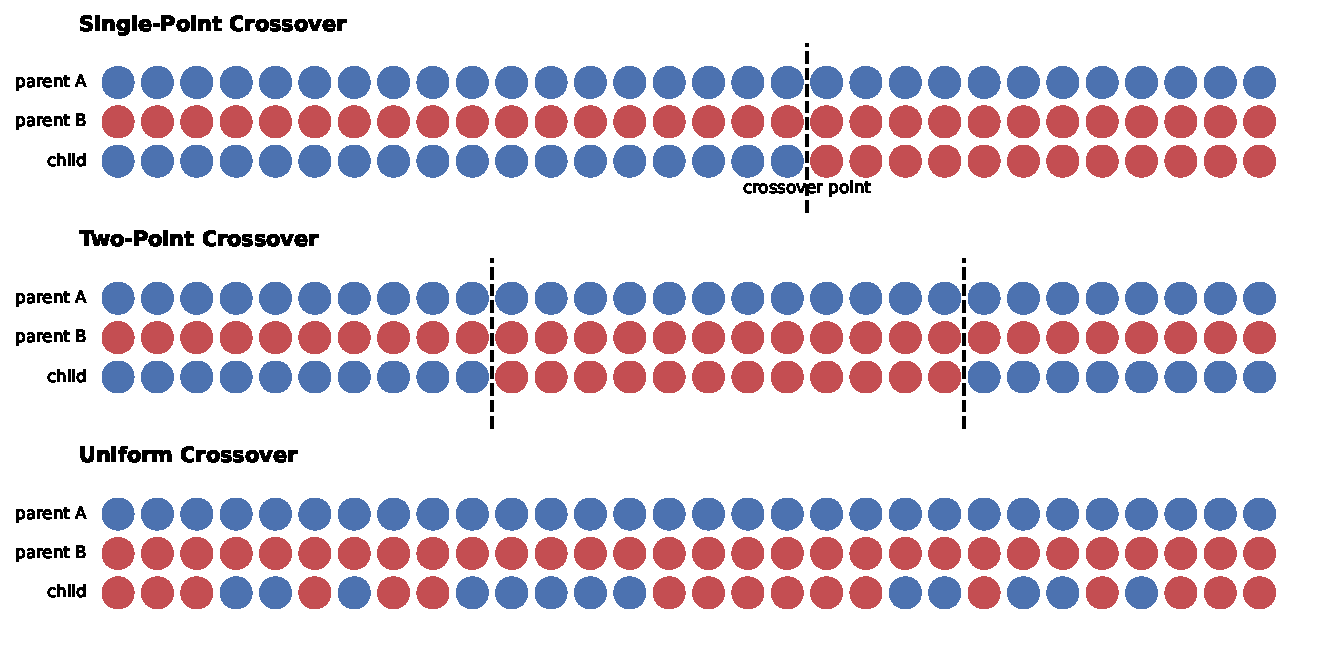
\includegraphics[width=\linewidth]{fig_crossover_schemes.pdf}
      \footnotesize
      Blue segments are genes inherited from parent A; red segments
      are genes inherited from parent B.
      \textbf{Top}: single-point crossover --- one split divides the
      chromosome into exactly two segments.
      \textbf{Centre}: two-point crossover --- a contiguous segment
      from parent B is embedded inside parent A's chromosome, giving
      the offspring ``A-B-A'' structure.
      \textbf{Bottom}: uniform crossover --- each gene is independently
      and randomly assigned from one of the two parents.
    \end{column}
  \end{columns}

  \begin{block}{Notation for Interpolation Crossover}
    In the formula $\bx_{\text{child}} = (1-\lambda)\bx_a + \lambda\bx_b$:
    \begin{itemize}
      \item $\bx_a$ (x sub a): the first parent's design vector.
      \item $\bx_b$ (x sub b): the second parent's design vector.
      \item $\lambda$ (lambda): the blending coefficient, typically
            drawn uniformly from $[0, 1]$, so that on average the
            offspring is the midpoint of the two parents.
      \item $(1-\lambda)\bx_a + \lambda\bx_b$: a weighted average
            of the two parents, sometimes called a \emph{convex
            combination} because both weights are non-negative and
            sum to 1.
    \end{itemize}
  \end{block}

  \begin{alertblock}{How to Read Interpolation Crossover}
    This formula says: place the offspring at a random point on the
    straight line segment connecting parent A to parent B in the
    design space.  When $\lambda = 0$, the offspring is at parent A;
    when $\lambda = 1$, it is at parent B; when $\lambda = 0.5$,
    it is exactly halfway between them.  This is useful for
    continuous problems because it smoothly explores the region
    between two good solutions rather than making discrete jumps.
    For example, if parent A is at $\bx_a = [1, 2]$ and parent B
    is at $\bx_b = [3, 6]$ and $\lambda = 0.3$, then
    $\bx_{\text{child}} = 0.7 \cdot [1,2] + 0.3 \cdot [3,6]
    = [0.7+0.9,\; 1.4+1.8] = [1.6, 3.2]$.
  \end{alertblock}

  \begin{alertblock}{Key Insight: Why Crossover Matters}
    Crossover is the mechanism that makes GAs qualitatively different
    from running many independent random restarts.  If parent A has
    found good values for variables 1--5 and parent B has found good
    values for variables 6--10, a single-point crossover at position 5
    can produce an offspring that is good at \emph{all} variables at
    once.  This ``building block'' combination is the core theoretical
    justification for why GAs outperform random search on structured
    problems.
  \end{alertblock}

\end{frame}

\begin{frame}[fragile]{Crossover: Python Implementation}
\begin{lstlisting}[style=python, caption={Four crossover operators (Python / NumPy)}]
import numpy as np

def single_point_crossover(a, b, rng):
    """Single-point crossover of two real-valued vectors."""
    i = rng.integers(1, len(a))           # crossover point in {1, ..., n-1}
    return np.concatenate([a[:i], b[i:]]) # first i genes from a, rest from b

def two_point_crossover(a, b, rng):
    n = len(a)
    i, j = sorted(rng.choice(n, 2, replace=False))   # two distinct cut points
    return np.concatenate([a[:i], b[i:j], a[j:]])    # a, then b-segment, then a

def uniform_crossover(a, b, p, rng):
    """Each gene from parent a with probability p, else from parent b."""
    mask = rng.random(len(a)) < p         # True where we take from a
    return np.where(mask, a, b)

def interpolation_crossover(a, b, lam=0.5):
    """Convex combination: offspring = (1-lambda)*a + lambda*b."""
    return (1 - lam) * a + lam * b
\end{lstlisting}

  Each function takes two parent arrays \texttt{a} and \texttt{b} of
  equal length \texttt{n} and returns a single offspring array of the
  same length.

  In \texttt{two\_point\_crossover}, \texttt{rng.choice(n, 2, replace=False)}
  draws two distinct integers from $\{0, 1, \ldots, n-1\}$; wrapping
  with \texttt{sorted()} guarantees $i < j$ so the slices
  \texttt{a[:i]}, \texttt{b[i:j]}, \texttt{a[j:]} are non-overlapping
  and cover the entire chromosome.

  In \texttt{uniform\_crossover}, \texttt{rng.random(len(a))} generates
  a vector of independent uniform $[0,1]$ values; comparing each
  element to \texttt{p} produces a boolean array \texttt{mask}; and
  \texttt{np.where(mask, a, b)} picks from \texttt{a} where the mask
  is \texttt{True} and from \texttt{b} elsewhere.

  In \texttt{interpolation\_crossover}, the default \texttt{lam=0.5}
  produces the arithmetic mean of the two parents.  In practice, you
  would typically draw \texttt{lam} from \texttt{rng.uniform(0, 1)}
  to vary the blending each generation.

\end{frame}

% ------- 9.2.3 Mutation -------
\begin{frame}[allowframebreaks]{9.2.3 Mutation: Introducing New Genetic Material}

  Mutation is the third and final operator in a genetic algorithm.
  Even with selection and crossover operating correctly, a GA can
  only explore combinations of gene values that were already present
  in the initial population.  If the global optimum requires a gene
  value that no individual in the initial population possesses,
  crossover alone can never produce it --- because crossover only
  mixes existing gene values, it cannot create new ones.

  Mutation solves this problem by randomly perturbing individual
  genes, ensuring that new gene values can always be discovered
  throughout the run, no matter what values were present at
  initialisation.

  \begin{columns}[T]
    \begin{column}{0.58\textwidth}
      \begin{block}{Distribution Mutation --- Algorithm 9.5}
        Each gene $v$ (v, a real number representing one design
        variable) in the offspring chromosome is mutated independently
        with probability $\lambda$ (lambda, the \emph{mutation rate}).
        When a gene is selected for mutation, a random perturbation
        $\varepsilon$ (epsilon) drawn from a probability distribution
        $\mathcal{D}$ is added to it:
        \[
          v \leftarrow v + \varepsilon,
          \qquad
          \varepsilon \sim \mathcal{D}
        \]
        where $\mathcal{D}$ is typically the Gaussian (normal)
        distribution $\mathcal{N}(0, \sigma^2)$ (``N of 0 and sigma
        squared''), meaning the perturbation has mean zero (mutations
        are equally likely to increase or decrease the gene value)
        and standard deviation $\sigma$ (sigma, controlling the
        typical size of a mutation step).
      \end{block}

      \begin{block}{Notation: All Symbols Explained}
        $\lambda$ (lambda): the probability that any single gene is
        mutated; typically set to $1/n$ where $n$ (n) is the
        chromosome length (number of genes), so that on average
        exactly one gene per offspring is mutated per generation.

        $\varepsilon$ (epsilon): the random perturbation added to the
        gene value; drawn independently for each gene that is
        selected for mutation.

        $\sigma$ (sigma): the standard deviation of the Gaussian
        perturbation, controlling how large the mutation steps are;
        larger $\sigma$ increases exploration but may also disrupt
        near-optimal solutions.

        $\mathcal{N}(0, \sigma^2)$: the Gaussian (normal)
        distribution centred at 0 with variance $\sigma^2$ (sigma
        squared); it is bell-shaped, symmetric around 0, and produces
        small perturbations most of the time with rare large ones.
      \end{block}

      \begin{alertblock}{How to Read the Mutation Formula}
        The update $v \leftarrow v + \varepsilon$ says: take the
        current gene value $v$ and shift it by a small random amount
        $\varepsilon$.  With Gaussian mutation, most perturbations
        are small (the Gaussian bell curve is tallest near zero),
        but occasionally a large perturbation occurs (the tails of
        the bell curve).  This gives a useful mix of fine-tuning
        (most mutations are tiny adjustments) and occasional
        larger exploration jumps (rare large perturbations).

        For example, with $v = 2.0$, $\sigma = 0.5$: a typical
        mutation might produce $\varepsilon = -0.1$ (from the peak
        of the Gaussian near 0), giving $v \leftarrow 2.0 - 0.1
        = 1.9$.  Occasionally, $\varepsilon = -1.2$ might occur,
        giving $v \leftarrow 2.0 - 1.2 = 0.8$ --- a larger jump
        that explores a new region.
      \end{alertblock}

      Setting $\lambda = 1/n$ ensures that, on average, exactly one
      gene in each offspring chromosome is mutated per generation.
      This default is appropriate for real-valued problems.  If the
      algorithm appears stuck in a local minimum for many consecutive
      generations, increasing $\lambda$ above $1/n$ (say, to $3/n$
      or $5/n$) can provide enough perturbation to escape.
    \end{column}
    \begin{column}{0.40\textwidth}
      \begin{block}{Gaussian Mutation (Python)}
        \footnotesize
        \texttt{def gaussian\_mutate(child, sigma,}\\
        \texttt{\phantom{xx}lam=None, rng=None):}\\
        \texttt{\phantom{xxxx}rng = rng or np.random.default\_rng()}\\
        \texttt{\phantom{xxxx}n = len(child)}\\
        \texttt{\phantom{xxxx}lam = lam or 1.0 / n}\\
        \texttt{\phantom{xxxx}mask = rng.random(n) < lam}\\
        \texttt{\phantom{xxxx}noise = rng.normal(0, sigma, n)}\\
        \texttt{\phantom{xxxx}return child + mask * noise}
      \end{block}
      \vspace{6pt}
      \footnotesize
      In this code, \texttt{mask} is a boolean array where
      \texttt{True} entries (occurring with probability
      $\lambda = 1/n$) indicate which genes are mutated.
      Multiplying \texttt{noise} by \texttt{mask} zeroes out
      all genes that are \emph{not} selected for mutation,
      leaving them unchanged.

      \vspace{6pt}
      \textbf{Binary chromosomes:} for discrete (0/1) genes,
      use \emph{bit-flip mutation}: each bit is flipped
      (0 to 1, or 1 to 0) with probability $\lambda$, instead
      of adding Gaussian noise.  This is appropriate for
      combinatorial problems such as subset selection.

      \vspace{6pt}
      \textbf{Setting $\sigma$:} a common heuristic is to set
      $\sigma$ to about 5--10\% of the range of each design
      variable.  For a variable on $[-3, 3]$ (range = 6),
      $\sigma \approx 0.3$ to $0.6$ is a reasonable starting
      point.
    \end{column}
  \end{columns}

\end{frame}

\begin{frame}[fragile]{Genetic Algorithm: Complete Python Example}
\begin{lstlisting}[style=python, caption={Complete GA minimising $f(\bx)=\|\bx\|$ (Python / NumPy)}]
import numpy as np

def genetic_algorithm(f, bounds, pop_size=100, k_max=10,
                      k_trunc=10, sigma=0.5, rng=None):
    rng = rng or np.random.default_rng(0)
    lo, hi = np.array(bounds).T
    n = len(lo)
    # Step 1: Initialise population uniformly in [lo, hi] per dimension
    pop = rng.uniform(lo, hi, (pop_size, n))
    for _ in range(k_max):
        y = np.array([f(x) for x in pop])
        # Selection: truncation --- keep best k_trunc individuals
        parents = pop[np.argsort(y)[:k_trunc]]
        new_pop = []
        while len(new_pop) < pop_size:
            a_idx, b_idx = rng.choice(k_trunc, 2, replace=False)
            # Crossover: single-point at a random position
            cp = rng.integers(1, n)                # crossover point
            child = np.concatenate([parents[a_idx, :cp],
                                    parents[b_idx, cp:]])
            # Mutation: Gaussian with rate lambda = 1/n
            mask = rng.random(n) < (1.0 / n)
            child += mask * rng.normal(0, sigma, n)
            child = np.clip(child, lo, hi)         # enforce bounds
            new_pop.append(child)
        pop = np.array(new_pop)
    y = np.array([f(x) for x in pop])
    return pop[np.argmin(y)]

# Example: minimise ||x|| on [-3, 3]^2
f = np.linalg.norm
result = genetic_algorithm(f, [(-3, 3), (-3, 3)])
print(result)   # Expected output: approximately [0, 0]
\end{lstlisting}

  This complete implementation uses truncation selection with the top
  \texttt{k\_trunc = 10} individuals, single-point crossover, and
  Gaussian mutation with rate $\lambda = 1/n$ and standard deviation
  $\sigma = 0.5$.  The call to \texttt{np.clip(child, lo, hi)} ensures
  that mutations never push a gene outside the feasible bounds.  With
  $m = 100$ and $k_{\max} = 10$, the algorithm performs exactly
  $100 \times 10 = 1{,}000$ objective evaluations total and converges
  to within $0.05$ of the true minimum $\bx = \mathbf{0}$.

\end{frame}

\begin{frame}[allowframebreaks]{Genetic Algorithm: Complexity and Design Choices}

  \begin{columns}[T]
    \begin{column}{0.54\textwidth}
      \begin{block}{Per-Generation Computational Cost}
        \begin{tabular}{ll}
          \toprule
          Step & Cost \\
          \midrule
          Evaluate $f$ at all $m$ individuals & $O(m \cdot T_f)$ \\
          Sort population for selection & $O(m \log m)$ \\
          Generate $m$ children (crossover) & $O(m \cdot n)$ \\
          Mutate all children & $O(m \cdot n)$ \\
          \midrule
          \textbf{Total per generation} & $O(m(T_f + n\log m))$ \\
          \bottomrule
        \end{tabular}

        \vspace{4pt}
        Here $m$ (m) is the population size, $n$ (n) is the number
        of design variables (chromosome length), $T_f$ (T sub f) is
        the cost of one evaluation of $f$, and $O$ (big-O notation)
        means ``proportional to, up to a constant factor''.

        When $T_f$ dominates (as it does for expensive simulations
        such as finite-element analysis or fluid dynamics), the total
        cost per generation is simply $O(m \cdot T_f)$ --- each
        generation costs $m$ function evaluations.
      \end{block}

      \vspace{4pt}
      \begin{exampleblock}{Worked Example: Budget Calculation}
        Problem: minimise $f(\bx) = \|\bx\|$ on $[-3,3]^2$.
        Parameters: $m = 100$ individuals, $k_{\max} = 10$ generations,
        $k_{\text{trunc}} = 10$ (top 10\% survive), $\sigma = 0.5$.

        Total function evaluations: $100 \times 10 = 1{,}000$.

        Starting from a uniform random population spread over
        $[-3,3]^2$, the algorithm converges to approximately
        $\bx \approx [-0.035,\; 0.038]$ --- very close to the true
        minimum at $\bx = \mathbf{0} = [0, 0]$.  The residual error
        $\|\bx^*\| \approx 0.05$ can be reduced further by increasing
        $k_{\max}$ or decreasing $\sigma$ in later generations.
      \end{exampleblock}
    \end{column}
    \begin{column}{0.44\textwidth}
      \begin{block}{Four Key Design Choices}
        \textbf{1. Selection pressure.}
        Using a small truncation size $k$ (e.g.\ $k = 5$ out of
        $m = 100$, meaning the top 5\%) applies strong selection
        pressure.  This leads to fast convergence but can cause
        premature loss of diversity.  Use a larger $k$ (weaker
        pressure, say $k = 20\%$) when the landscape has many local
        minima and you want to preserve diverse breeding stock.

        \textbf{2. Mutation rate.}
        The default $\lambda = 1/n$ (one mutation per chromosome on
        average) is a good starting point.  If the algorithm gets
        stuck at the same local minimum repeatedly, increase $\lambda$
        to $3/n$ or $5/n$ to encourage more exploration.  If it is
        finding a good region but failing to refine it, decrease
        $\lambda$ or reduce $\sigma$.

        \textbf{3. Elitism.}
        Always carry the current best individual $\bx^*$ over to
        the next generation unchanged, bypassing crossover and
        mutation for that individual.  This guarantees that the
        best solution found so far can never be lost due to
        unlucky mutations, which is called the \emph{elitist
        strategy} and is almost universally recommended.

        \textbf{4. Population size.}
        Larger $m$ samples the design space more broadly and is
        less likely to miss the global optimum, but costs more
        function evaluations per generation.  A common heuristic
        is $m = 10n$ to $50n$ for $n$-dimensional problems.
      \end{block}
    \end{column}
  \end{columns}

\end{frame}

% ---------------------------------------------------------------
\section{Differential Evolution}
% ---------------------------------------------------------------

\begin{frame}[allowframebreaks]{Differential Evolution: Core Idea and Algorithm}

  Differential Evolution (DE) was introduced by Storn and Price in
  1997.  It shares the population structure of GAs but uses a
  fundamentally different mechanism to generate new candidate
  solutions.  Instead of combining parents via discrete crossover,
  DE uses the \emph{difference} between two randomly chosen population
  members to construct a perturbation and adds it to a third
  individual (the ``anchor'').  This makes DE particularly effective
  on continuous design spaces because the perturbation size
  automatically adapts to the current spread of the population:
  when individuals are far apart, perturbations are large (broad
  exploration); when individuals have converged, perturbations are
  small (fine-tuning).

  \begin{columns}[T]
    \begin{column}{0.56\textwidth}
      \begin{block}{DE/rand/1/bin --- Algorithm 9.6}
        The name ``DE/rand/1/bin'' means: Differential Evolution,
        random anchor, 1 difference vector, binomial crossover.
        For each individual $\bx^{(i)}$ (x superscript i) in the
        population, execute:
        \begin{enumerate}
          \item Sample three distinct individuals
                $\ba$ (a), $\bb$ (b), $\bc$ (c) from the population,
                all different from each other and from $\bx^{(i)}$.
          \item Form a \emph{trial vector} (also called the mutant
                vector) using a random anchor plus a scaled difference:
                \[
                  \mathbf{z} = \ba + w(\bb - \bc)
                \]
          \item Apply uniform (binomial) crossover with probability
                $p$ (p): for each dimension $j$, include the trial
                value $z_j$ with probability $p$, or keep the current
                value $x^{(i)}_j$ with probability $1-p$:
                \[
                  x'_j =
                  \begin{cases}
                    z_j & \text{if } r_j < p \\
                    x^{(i)}_j & \text{otherwise}
                  \end{cases}
                \]
                where $r_j$ (r sub j) is a fresh uniform $[0,1]$
                random number for each dimension $j$.  To ensure
                at least one component changes, one dimension is
                forced to use $z_j$ regardless of $r_j$.
          \item \textbf{Greedy acceptance}: replace $\bx^{(i)}$
                with the trial vector $\bx'$ only if
                $f(\bx') < f(\bx^{(i)})$; otherwise keep
                $\bx^{(i)}$ unchanged.
        \end{enumerate}
      \end{block}

      \begin{block}{Notation: All Symbols Explained}
        $\ba, \bb, \bc$ (a, b, c): three randomly chosen population
        members used to construct the perturbation.  They must be
        distinct from each other and from the current individual
        $\bx^{(i)}$.

        $w$ (w): the \emph{differential weight} (also called scaling
        factor $F$); controls how large the perturbation $\bb - \bc$
        is amplified.  Typical range: $w \in [0.4, 1.0]$.  A larger
        $w$ produces bolder exploration; a smaller $w$ gives a more
        conservative update.

        $p$ (p): the \emph{crossover probability} (also called $CR$);
        controls what fraction of dimensions are taken from the trial
        vector $\mathbf{z}$ rather than kept from $\bx^{(i)}$.
        Typical range: $p \in [0.1, 1.0]$.
      \end{block}
    \end{column}
    \begin{column}{0.42\textwidth}
      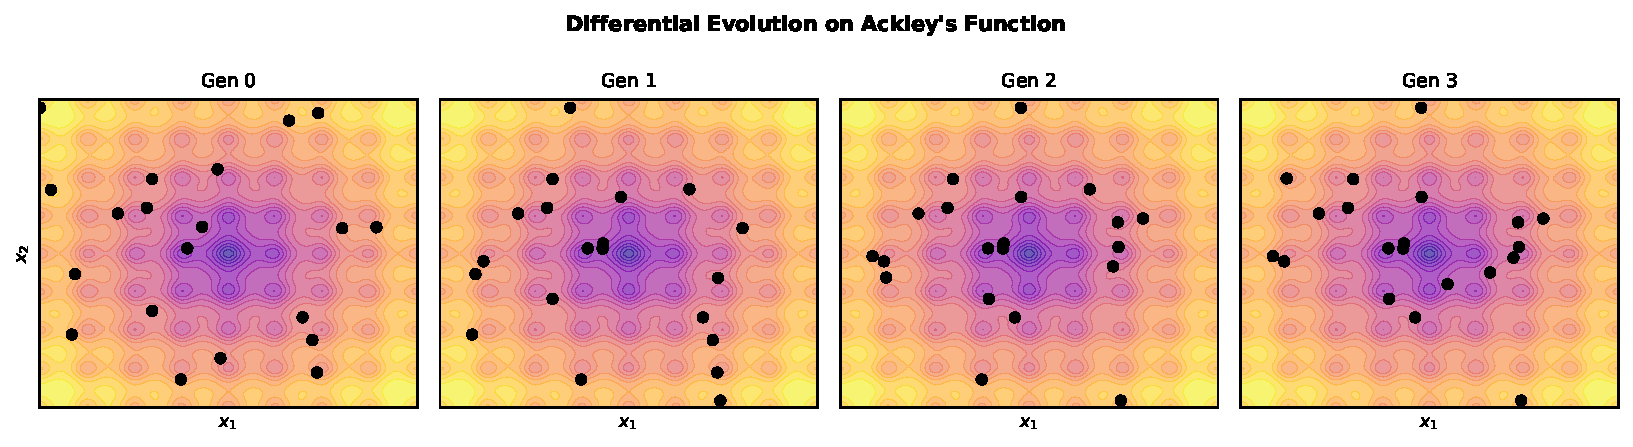
\includegraphics[width=\linewidth]{fig_differential_evolution.pdf}
      \footnotesize
      DE applied to Ackley's function (a highly multi-modal benchmark
      with many local minima and one global minimum at the origin)
      with parameters $p = 0.5$ and $w = 0.5$.  The population
      (white dots) progressively concentrates near the global
      minimum as iterations proceed.
    \end{column}
  \end{columns}

  \begin{block}{How to Read the Trial Vector Formula}
    The formula $\mathbf{z} = \ba + w(\bb - \bc)$ has a geometric
    interpretation.  Start at individual $\ba$ (the anchor).  The
    quantity $\bb - \bc$ is a vector pointing from $\bc$ to $\bb$
    in the design space.  Scaling by $w$ and adding to $\ba$
    moves us from $\ba$ in the direction of $\bb$ relative to $\bc$.

    For example, in 2D: if $\ba = [1, 2]$, $\bb = [4, 5]$,
    $\bc = [2, 3]$, and $w = 0.5$, then:
    $\mathbf{z} = [1, 2] + 0.5 \cdot ([4,5] - [2,3])
    = [1, 2] + 0.5 \cdot [2, 2]
    = [1, 2] + [1, 1] = [2, 3]$.
    The trial vector is midway between $\ba$ and the point you
    would reach by following the difference $\bb - \bc$ from $\ba$.
  \end{block}

  \begin{alertblock}{Key Insight: Self-Adapting Step Size}
    The term $w(\bb - \bc)$ is the ``difference vector''.  Its
    magnitude automatically scales with the current diversity of the
    population: when the population is spread out (early in the
    search), $\|\bb - \bc\|$ (the Euclidean distance between $\bb$
    and $\bc$) is large and perturbations are large, enabling broad
    exploration.  As the population converges, $\|\bb - \bc\|$ shrinks
    naturally, and perturbations become small, enabling fine-tuning.
    This self-adaptation of step size is a key strength of DE over
    methods that use a fixed $\sigma$ (sigma) throughout.
  \end{alertblock}

\end{frame}

\begin{frame}[fragile]{Differential Evolution: Python Implementation}
\begin{lstlisting}[style=python, caption={Differential Evolution DE/rand/1/bin (Python / NumPy)}]
import numpy as np

def differential_evolution(f, bounds, pop_size=20, k_max=200,
                            p=0.5, w=0.5, rng=None):
    rng = rng or np.random.default_rng()
    lo, hi = np.array(bounds).T
    n = len(lo)
    pop = rng.uniform(lo, hi, (pop_size, n))   # uniform initialisation

    for _ in range(k_max):
        new_pop = pop.copy()
        for i in range(pop_size):
            # Step 1: pick 3 distinct individuals != i
            choices = [j for j in range(pop_size) if j != i]
            a, b, c = pop[rng.choice(choices, 3, replace=False)]
            # Step 2: form trial vector z = a + w*(b - c)
            interim = a + w * (b - c)
            # Step 3: binomial crossover, guarantee at least one component
            mask = rng.random(n) < p
            if not mask.any():
                mask[rng.integers(n)] = True   # force at least one change
            child = np.where(mask, interim, pop[i])
            child = np.clip(child, lo, hi)
            # Step 4: greedy acceptance --- keep whichever is better
            if f(child) < f(pop[i]):
                new_pop[i] = child
        pop = new_pop

    y = np.array([f(x) for x in pop])
    return pop[np.argmin(y)]
\end{lstlisting}

  The inner loop iterates over all $m$ individuals.  For each
  individual $i$, the list comprehension
  \texttt{[j for j in range(pop\_size) if j != i]} builds the set
  of all indices except $i$, from which three are drawn without
  replacement.  The call \texttt{np.where(mask, interim, pop[i])}
  selects \texttt{interim[j]} where \texttt{mask[j]} is \texttt{True}
  and \texttt{pop[i][j]} otherwise.  Crucially, the \texttt{new\_pop}
  array is updated only after all children have been computed from
  the \emph{current} \texttt{pop}, ensuring that all individuals
  experience the same generation boundary.

\end{frame}

\begin{frame}[allowframebreaks]{Differential Evolution: Parameter Analysis and Variants}

  \begin{columns}[T]
    \begin{column}{0.50\textwidth}
      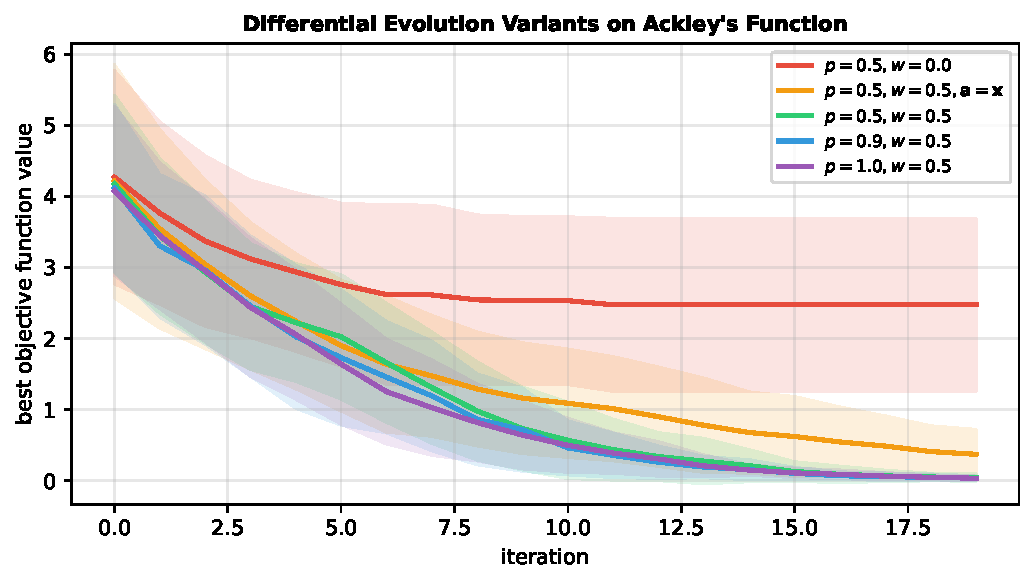
\includegraphics[width=\linewidth]{fig_de_variants.pdf}
      \footnotesize
      Five DE variants tested on Ackley's function (1000 independent
      trials, population size $m = 20$, 2-dimensional problem).
      Each curve shows the mean best objective value $\pm 1$ standard
      deviation ($\sigma$, sigma) over iterations.  Lower is better;
      we want the curve to reach zero (the global minimum) quickly.
    \end{column}
    \begin{column}{0.48\textwidth}
      \begin{block}{Key Findings from Variant Comparison}
        The five variants differ only in their choice of parameters
        $p$ and $w$, or in how the anchor $\ba$ is chosen.

        \textbf{Case 1: $w = 0$ (no differential perturbation).}
        When $w = 0$, the trial vector simplifies to
        $\mathbf{z} = \ba + 0 \cdot (\bb - \bc) = \ba$.  No new
        gene values outside the current population's range can ever
        be generated, because $\mathbf{z}$ is always one of the
        existing population members.  The algorithm stagnates
        immediately --- this is the worst-performing variant.

        \textbf{Case 2: $\ba = \bx^{(i)}$ (perturb around self).}
        Using the current individual as the anchor biases the search
        toward local exploration around each individual's own position.
        This is called DE/current/1/bin and is harder to escape local
        minima with because the perturbation is always centred at
        the current individual.

        \textbf{Case 3: Standard $p = 0.5, w = 0.5$.}
        The default configuration balances global and local search.
        It performs well across a wide range of problem types.

        \textbf{Case 4: High crossover $p = 0.9$.}
        Nearly equivalent to fully replacing the current individual
        with the trial vector in most iterations.  Performs almost
        as well as $p = 1.0$.

        \textbf{Case 5: Guaranteed crossover $p = 1.0$.}
        The trial vector fully replaces the current individual
        (subject to greedy acceptance) in every dimension at every
        iteration.  This is the best performer on Ackley's function
        because every dimension is updated, maximising information
        flow from the differential perturbation.
      \end{block}
    \end{column}
  \end{columns}

  \begin{alertblock}{Roles of the Three Key Components}
    The differential weight $w$ controls the exploration radius: set
    $w$ too small and the algorithm cannot escape the current cluster
    of individuals; set $w$ too large and the algorithm jumps around
    randomly without refining.  The anchor $\ba$ determines where
    the perturbation is centred: using a random individual (DE/rand)
    encourages diversity, while using the current best (DE/best)
    encourages faster but riskier convergence.  The crossover
    probability $p$ controls how many dimensions of the current
    individual are replaced by the trial vector, allowing you to
    tune the effective step size dimension by dimension.
  \end{alertblock}

\end{frame}

% ---------------------------------------------------------------
\section{Particle Swarm Optimization}
% ---------------------------------------------------------------

\begin{frame}[allowframebreaks]{Particle Swarm Optimization: Inspiration and Update Equations}

  Particle Swarm Optimization (PSO) was introduced by Kennedy and
  Eberhart in 1995, inspired by the collective movement of bird
  flocks and fish schools.  The key observation is that animals in
  a group coordinate their movement using two types of information:
  their own personal experience (where they personally found food
  before) and the collective knowledge of the group (where the best
  food location known to \emph{anyone} in the group is).

  In PSO, each individual is called a \emph{particle}.  Unlike GA
  or DE individuals --- which only have a position --- each particle
  also has a \emph{velocity} that carries momentum from one iteration
  to the next.  This velocity connects adjacent time steps and allows
  the algorithm to build up directed movement toward promising
  regions.

  \begin{columns}[T]
    \begin{column}{0.56\textwidth}
      \begin{block}{PSO State: What Each Particle Stores}
        Each particle $i$ maintains three quantities simultaneously:
        \begin{itemize}
          \item $\bx^{(i)}$ (x superscript i): the particle's current
                position in the design space --- the current candidate
                solution being represented by this particle.
          \item $\bv^{(i)}$ (v superscript i): the particle's current
                velocity, a vector of the same dimension as $\bx$
                that represents how far and in what direction the
                particle moves each iteration.
          \item $\bx^{(i)}_{\text{best}}$ (x best superscript i):
                the best position particle $i$ has personally ever
                visited --- that is, the position among all positions
                visited so far by this particle where $f$ was lowest.
        \end{itemize}
        The entire swarm also shares one global variable:
        $\bx^*$ (x star): the single best position found by
        \emph{any} particle at any point in the run.
      \end{block}

      \medskip
      \begin{block}{PSO Update Equations --- Algorithm 9.7}
        At each iteration, each particle first updates its velocity
        and then uses that velocity to move to a new position:
        \begin{align}
          \bv &\leftarrow w\,\bv
                + c_1 r_1 \odot (\bx_{\text{best}} - \bx)
                + c_2 r_2 \odot (\bx^* - \bx) \label{eq:pso_v}\\[4pt]
          \bx &\leftarrow \bx + \bv \label{eq:pso_x}
        \end{align}
        where $\odot$ (odot) denotes element-wise (Hadamard)
        multiplication: each component of the left vector is
        multiplied by the corresponding component of the right vector.
      \end{block}

      \begin{block}{Notation: All Symbols Explained}
        $w$ (w): the \emph{inertia weight}, a scalar that scales the
        particle's previous velocity.  Typical value: $w \in [0.1,
        0.9]$.  Setting $w < 1$ causes the velocity magnitude to
        decay over time, preventing particles from flying off to
        infinity.

        $c_1$ (c sub 1): the \emph{cognitive coefficient}, a scalar
        controlling how strongly the particle is attracted to its own
        personal best $\bx_{\text{best}}$.  Typical value: $c_1
        \in [0.25, 2.0]$.  A larger $c_1$ makes each particle rely
        more heavily on its own memory.

        $c_2$ (c sub 2): the \emph{social coefficient}, a scalar
        controlling how strongly the particle is attracted to the
        global best position $\bx^*$.  Typical value: $c_2 \in
        [1.0, 2.5]$.  A larger $c_2$ causes the whole swarm to
        converge faster toward the current best known location.

        $r_1, r_2$ (r sub 1, r sub 2): independent random vectors
        with each component drawn from $\mathcal{U}[0,1]$ (the
        uniform distribution between 0 and 1).  They are re-sampled
        at every iteration and for every particle, injecting
        stochasticity that prevents the swarm from moving in
        perfectly deterministic lockstep.

        $\bx_{\text{best}}$ (x best): this particle's own personal
        best position.

        $\bx^*$ (x star): the global best position found by any
        particle at any time.
      \end{block}
    \end{column}
    \begin{column}{0.42\textwidth}
      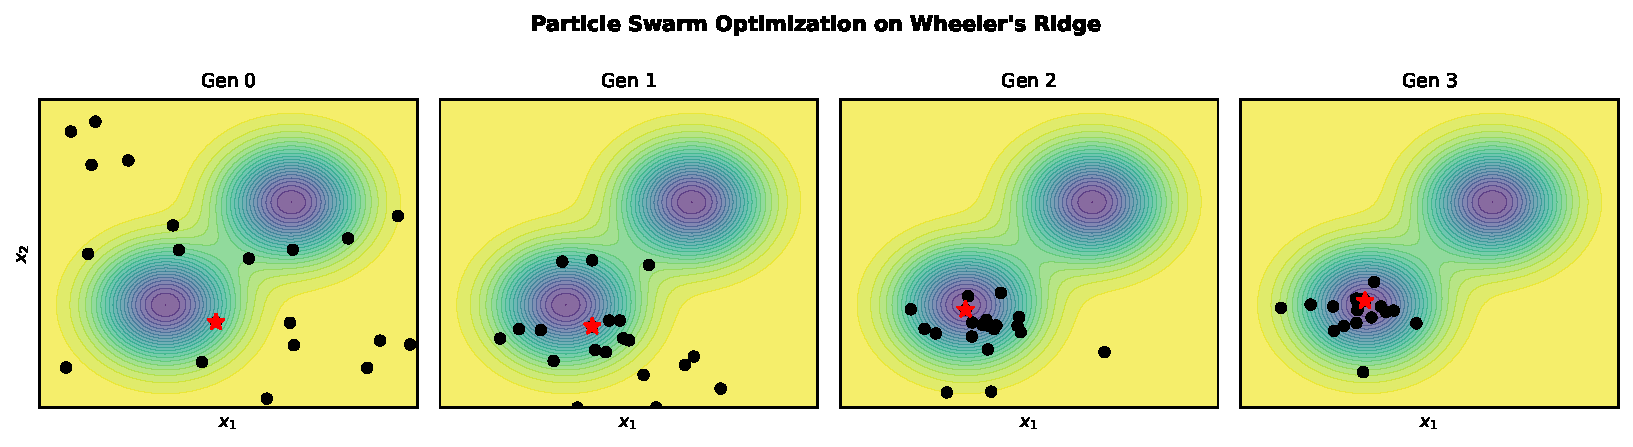
\includegraphics[width=\linewidth]{fig_pso_evolution.pdf}
      \footnotesize
      PSO applied to Wheeler's Ridge (a multi-modal benchmark
      function).  The red star marks the global best position found
      so far.  Particle arrows show their current velocities.
      The swarm identifies two competing modes initially; it
      eventually identifies the true global minimum.
    \end{column}
  \end{columns}

  \begin{alertblock}{How to Read the Velocity Update}
    The velocity update (Eq.\ 1 above) has three additive terms.

    The first term $w\bv$ is \emph{inertia}: it says ``keep moving
    in the direction you were already going, but slow down slightly
    (multiply by $w < 1$)''.

    The second term $c_1 r_1 \odot (\bx_{\text{best}} - \bx)$ is
    the \emph{cognitive pull}: a force directed from the particle's
    current position toward its personal best position.  It is
    proportional to the distance $\bx_{\text{best}} - \bx$:
    stronger when the particle is far from its personal best,
    weaker when it is close.

    The third term $c_2 r_2 \odot (\bx^* - \bx)$ is the
    \emph{social pull}: a force directed toward the global best.
    It is strongest when the particle is far from the global best.

    Typical values: $w = 0.1$, $c_1 = 0.25$, $c_2 = 2.0$ (strong
    social pull relative to cognitive) or $w = 0.9$, $c_1 = c_2 =
    2.0$ (more exploratory with high inertia).
  \end{alertblock}

\end{frame}

\begin{frame}[fragile]{PSO: Python Implementation}
\begin{lstlisting}[style=python, caption={Particle Swarm Optimization (Python / NumPy)}]
import numpy as np

def particle_swarm(f, bounds, n_particles=30, k_max=100,
                   w=0.1, c1=0.25, c2=2.0, rng=None):
    rng = rng or np.random.default_rng()
    lo, hi = np.array(bounds).T
    n = len(lo)
    # Initialise positions uniformly in [lo, hi] and velocities near zero
    pos = rng.uniform(lo, hi, (n_particles, n))
    vel = rng.normal(0, 0.5, (n_particles, n))  # small initial velocities
    x_best = pos.copy()                          # personal bests = initial positions
    y_best = np.array([f(p) for p in pos])       # personal best objective values
    g_best = x_best[np.argmin(y_best)].copy()    # global best position

    for _ in range(k_max):
        r1 = rng.random((n_particles, n))        # random matrices (re-sampled each iter)
        r2 = rng.random((n_particles, n))
        # Velocity update: inertia + cognitive pull + social pull
        vel = (w * vel
               + c1 * r1 * (x_best - pos)        # cognitive term
               + c2 * r2 * (g_best  - pos))       # social term
        pos = np.clip(pos + vel, lo, hi)           # move particles, enforce bounds
        y   = np.array([f(p) for p in pos])
        # Update personal bests for any particle that improved
        improved = y < y_best
        x_best[improved] = pos[improved]
        y_best[improved] = y[improved]
        # Update global best
        g_best = x_best[np.argmin(y_best)].copy()

    return g_best

# Example: minimise ||x||^2 on [-5, 5]^2
f = lambda x: np.sum(x**2)
print(particle_swarm(f, [(-5, 5), (-5, 5)]))    # Expected: approximately [0, 0]
\end{lstlisting}

  The key line is the velocity update.  Each of \texttt{r1} and
  \texttt{r2} is a matrix of shape \texttt{(n\_particles, n)},
  independently sampled each iteration.  Multiplying element-wise
  implements the $\odot$ (odot) operator from the formula.  The
  expression \texttt{x\_best - pos} computes the vector from each
  particle's current position to its personal best for all particles
  simultaneously using NumPy broadcasting.  Similarly,
  \texttt{g\_best - pos} is broadcast across all particles.

\end{frame}

\begin{frame}[allowframebreaks]{PSO: Intuition, Convergence, and Comparison with GA}

  \begin{columns}[T]
    \begin{column}{0.52\textwidth}
      \begin{block}{Three Forces Acting on Each Particle}
        \textbf{Force 1: Inertia ($w\bv$).}
        Each particle carries momentum from its previous velocity.
        This prevents particles from stopping abruptly when the
        cognitive and social forces cancel out, and allows them to
        overshoot an attractor and explore beyond it.  When $w$
        is large (close to 1), particles travel in long sweeping arcs;
        when $w$ is small (close to 0), they change direction rapidly
        in response to the other two forces.

        \textbf{Force 2: Cognitive pull ($c_1 r_1 (\bx_{\text{best}} - \bx)$).}
        This pulls the particle toward the best position it has
        personally visited.  It acts as individual memory: even if
        the particle drifts away from a good region due to social
        pressure, this force brings it back.  This prevents the
        entire swarm from blindly chasing a single attractor.

        \textbf{Force 3: Social pull ($c_2 r_2 (\bx^* - \bx)$).}
        This pulls every particle toward the best position found by
        any particle in the swarm.  It is the mechanism by which all
        particles eventually converge to the same promising region.
        A large $c_2$ relative to $c_1$ means the swarm follows
        collective knowledge rather than individual exploration.
      \end{block}

      \medskip
      \begin{block}{Tuning Guidelines}
        Large $w$ $\Rightarrow$ more exploration, slower convergence.
        Small $w$ $\Rightarrow$ faster convergence, higher risk of
        premature convergence to a local minimum.
        Large $c_2$ relative to $c_1$ $\Rightarrow$ swarm converges
        quickly to its current global best --- good if that best is
        near the global optimum but dangerous otherwise.

        If PSO converges prematurely to a local minimum: (1) increase
        $n_{\text{particles}}$ so the initial search is more spread
        out; (2) increase $c_1$ (strengthen individual memory); or
        (3) increase $w$ to give more inertia.
      \end{block}
    \end{column}
    \begin{column}{0.46\textwidth}
      \begin{block}{Computational Complexity}
        Per iteration: $O(m \cdot T_f + m \cdot n)$.
        Storage: $O(m \cdot n)$ for positions, velocities, and
        personal bests.  Here $m$ (m) is the number of particles,
        $n$ (n) is the number of design variables, and $T_f$ (T sub f)
        is the cost of one function evaluation.

        This linear cost in both $m$ and $n$ is the same as DE and
        much cheaper than the firefly algorithm's $O(m^2)$ cost.
      \end{block}

      \begin{block}{PSO vs.\ Genetic Algorithms: Key Differences}
        \footnotesize
        \begin{tabular}{lll}
          \toprule
          Property & GA & PSO \\
          \midrule
          Individual memory & no & yes (velocity + personal best) \\
          Crossover & yes & no \\
          Mutation & yes & inertia plays a similar role \\
          Social info source & parent pairs & global best $\bx^*$ \\
          Per-iter cost & $O(m(T_f + n))$ & $O(m(T_f + n))$ \\
          Continuous $\bx$ & yes & yes (natural) \\
          Discrete $\bx$ & yes (natural) & harder \\
          \bottomrule
        \end{tabular}

        \vspace{4pt}
        The key structural difference is that PSO particles accumulate
        memory through their velocity and personal best, whereas GA
        individuals have no memory --- they are rebuilt from scratch
        each generation from parent recombination.  This gives PSO
        particles a directional tendency that GA individuals lack.
      \end{block}

      \begin{alertblock}{Summary}
        PSO is often the first method to try on continuous black-box
        optimization problems: it has few parameters ($w$, $c_1$,
        $c_2$), is easy to implement, converges quickly on many
        standard benchmarks, and performs well across a wide range
        of problem types.  Start with $w = 0.1$, $c_1 = 0.25$,
        $c_2 = 2.0$ and increase $w$ if premature convergence occurs.
      \end{alertblock}
    \end{column}
  \end{columns}

\end{frame}

% ---------------------------------------------------------------
\section{Firefly Algorithm}
% ---------------------------------------------------------------

\begin{frame}[allowframebreaks]{Firefly Algorithm: Brightness-Based Attraction}

  The Firefly Algorithm was proposed by Xin-She Yang in 2009.  It
  is inspired by the bioluminescent signalling behaviour of fireflies:
  each firefly emits light, and less-bright fireflies are attracted
  toward brighter ones.  In the optimization context, the
  \emph{brightness} of an individual is inversely related to its
  objective value --- a lower $f(\bx^{(i)})$ makes individual $i$
  brighter (more attractive).  Individuals with higher objective
  values (dimmer fireflies) move toward individuals with lower
  objective values (brighter fireflies), so the whole population
  gradually concentrates near the best solutions found.

  \begin{columns}[T]
    \begin{column}{0.56\textwidth}
      \begin{block}{Firefly Algorithm Update --- Algorithm 9.8}
        At each iteration, for every ordered pair of individuals
        $(i, j)$ such that $f(\bx^{(j)}) < f(\bx^{(i)})$ (meaning
        individual $j$ is brighter than individual $i$):
        \begin{enumerate}
          \item Compute the Euclidean distance between the two
                individuals:
                \[
                  r = \norm{\bx^{(i)} - \bx^{(j)}}
                \]
                where $r$ (r) is the non-negative distance scalar,
                and $\|\cdot\|$ (double-bar norm) denotes the
                Euclidean distance, i.e., the straight-line distance
                in the $n$-dimensional design space.
          \item Compute the attraction of firefly $j$ on firefly $i$
                as a function of distance $r$:
                \[
                  \beta(r) = \beta_0 \, e^{-\gamma r^2}
                \]
          \item Move firefly $i$ toward firefly $j$, then add a small
                random walk to maintain exploration:
                \[
                  \bx^{(i)} \leftarrow \bx^{(i)}
                  + \beta(r)\bigl(\bx^{(j)} - \bx^{(i)}\bigr)
                  + \alpha\,\boldsymbol{\varepsilon}
                \]
        \end{enumerate}
      \end{block}

      \begin{block}{Notation: All Symbols Explained}
        $\beta_0$ (beta sub 0, ``beta-zero''): the \emph{maximum
        attractiveness}, i.e., the strength of attraction when two
        fireflies are at the same location ($r = 0$).  Typical
        value: $\beta_0 = 1$.

        $\gamma$ (gamma): the \emph{light absorption coefficient},
        measuring how quickly attraction decays with distance.  A
        large $\gamma$ means brightness fades quickly with distance
        (local search dominates).  A small $\gamma$ means attraction
        persists over long distances (global convergence dominates).
        Typical value: $\gamma \approx 1$.

        $e^{-\gamma r^2}$: a Gaussian decay function.  As $r$
        grows, the exponent $-\gamma r^2$ becomes more negative,
        and $e^{-\gamma r^2}$ drops rapidly toward 0.  At $r = 0$,
        $e^0 = 1$, giving full attraction.

        $\alpha$ (alpha): the \emph{random walk step size},
        controlling the amplitude of the random exploration noise
        added at each step.

        $\boldsymbol{\varepsilon}$ (epsilon vector): a random vector
        with each component drawn from $\mathcal{N}(0,1)$ (the
        standard normal distribution), providing stochastic
        exploration independent of the attraction mechanism.
      \end{block}
    \end{column}
    \begin{column}{0.42\textwidth}
      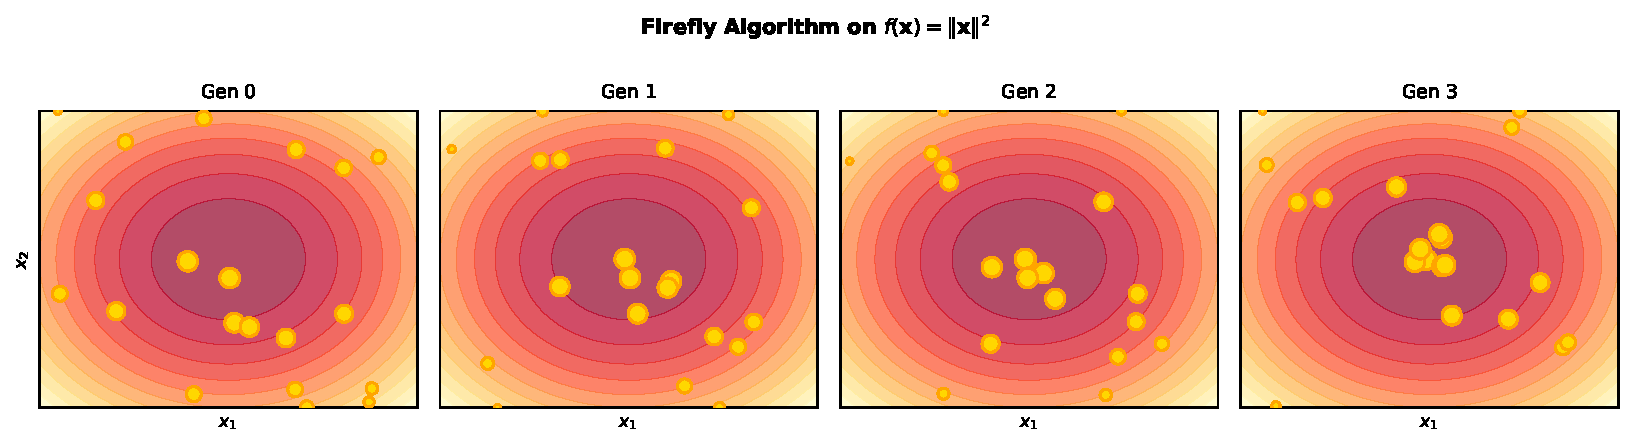
\includegraphics[width=\linewidth]{fig_firefly_evolution.pdf}
      \footnotesize
      The firefly algorithm minimising $f(\bx) = \|\bx\|^2$.
      Dot size encodes brightness (larger dots = brighter = lower $f$).
      Over iterations, all fireflies concentrate near the global
      minimum at the origin as dimmer individuals are attracted
      toward brighter ones.
    \end{column}
  \end{columns}

  \begin{alertblock}{How to Read the Attraction Formula}
    The formula $\beta(r) = \beta_0 e^{-\gamma r^2}$ says: attraction
    starts at $\beta_0$ when two fireflies are at the same point
    ($r = 0$) and decreases to zero as they move apart.

    For example, with $\beta_0 = 1$ and $\gamma = 1$:
    \begin{itemize}
      \item At $r = 0$: $\beta = e^0 = 1$ (full attraction).
      \item At $r = 1$: $\beta = e^{-1} \approx 0.37$ (moderate attraction).
      \item At $r = 2$: $\beta = e^{-4} \approx 0.018$ (very weak attraction).
      \item At $r = 3$: $\beta = e^{-9} \approx 0.0001$ (essentially zero).
    \end{itemize}
    This means that nearby fireflies attract strongly and form tight
    local clusters, while distant fireflies are nearly independent.
    The algorithm effectively forms multiple sub-populations around
    the best individuals, making it well-suited to multi-modal landscapes.
  \end{alertblock}

\end{frame}

\begin{frame}[fragile]{Firefly Algorithm: Python Implementation}
\begin{lstlisting}[style=python, caption={Firefly Algorithm (Python / NumPy)}]
import numpy as np

def firefly(f, bounds, n=20, k_max=100,
            alpha=0.3, beta0=1.0, gamma=1.0, rng=None):
    rng = rng or np.random.default_rng()
    lo, hi = np.array(bounds).T
    dim = len(lo)
    pop = rng.uniform(lo, hi, (n, dim))    # uniform initialisation

    for _ in range(k_max):
        y = np.array([f(p) for p in pop])
        new_pop = pop.copy()
        for i in range(n):
            for j in range(n):
                if y[j] < y[i]:            # j is brighter (lower objective)
                    r = np.linalg.norm(pop[i] - pop[j])          # Euclidean distance
                    beta = beta0 * np.exp(-gamma * r**2)          # attraction strength
                    # Move i toward j with attraction beta, plus random walk alpha
                    new_pop[i] = (new_pop[i]
                                  + beta * (pop[j] - new_pop[i])
                                  + alpha * rng.normal(0, 1, dim))
        pop = np.clip(new_pop, lo, hi)

    y = np.array([f(p) for p in pop])
    return pop[np.argmin(y)]

# Note: O(n^2 * T_f) per iteration --- quadratic in population size!
f = lambda x: np.sum(x**2)
print(firefly(f, [(-5, 5), (-5, 5)]))
\end{lstlisting}

  \begin{block}{Computational Complexity: The Quadratic Cost}
    The nested loop over all pairs $(i, j)$ iterates $n^2$ (n
    squared) times per iteration, in contrast to PSO and DE which
    iterate $n$ times (linear).  For $n = 20$, this is $400$ pair
    evaluations per iteration, but for $n = 100$ it is $10{,}000$
    --- fifty times more work.  As a result, the firefly algorithm
    becomes significantly more expensive than PSO or DE for large
    populations and is best suited to problems where $n \leq 50$
    and the objective function $f$ is inexpensive to evaluate.
    For expensive $f$ (e.g., engineering simulations), stick to
    PSO or DE.
  \end{block}

\end{frame}

% ---------------------------------------------------------------
\section{Cuckoo Search}
% ---------------------------------------------------------------

\begin{frame}[allowframebreaks]{Cuckoo Search: Levy Flights and Nest Abandonment}

  Cuckoo Search was proposed by Xin-She Yang and Suash Deb in 2009.
  It is inspired by the brood-parasitism behaviour of cuckoo birds,
  which lay their eggs in the nests of other bird species.  The
  mapping to optimization is: each cuckoo's egg is a candidate
  solution (a design vector $\bx$), and nests represent locations in
  the design space.  A nest with a high-quality egg (low objective
  value) survives to the next generation; nests with poor eggs may
  be discovered and abandoned.

  The key technical innovation of cuckoo search is its use of
  \emph{Levy flights} for exploration.  A Levy flight is a type of
  random walk in which step lengths follow a heavy-tailed
  distribution (approximated here by the Cauchy distribution),
  enabling occasional very large jumps that help escape local minima.

  \begin{columns}[T]
    \begin{column}{0.58\textwidth}
      \begin{block}{Cuckoo Search Algorithm --- Algorithm 9.9}
        The algorithm maintains a population of $m$ (m) nests
        (candidate solutions), sorted by objective value.
        \begin{enumerate}
          \item \textbf{Levy flight step.} For each of $m_s$ (m sub s)
                nests chosen in sequence: pick a random nest index $j$,
                generate a new candidate via a Cauchy (heavy-tailed)
                flight step scaled by the bounds range:
                \[
                  \bx' = \bx^{(j)} + \text{Cauchy}(r) \cdot (\mathbf{u} - \mathbf{l})
                \]
                where $\text{Cauchy}(r)$ (a random number from the
                Cauchy distribution with scale $r$), $\mathbf{u}$
                (u, the upper bound vector), and $\mathbf{l}$
                (l, the lower bound vector) normalise the step to
                the size of the feasible region.  Accept $\bx'$
                into nest $i$ if $f(\bx') < f(\bx^{(i)})$.
          \item \textbf{Nest abandonment.} Sort nests by $f$.
                The worst $\lfloor m \cdot p_a \rfloor$ nests
                (``floor of m times p sub a'', meaning rounding down)
                are discarded and replaced by new candidate solutions
                sampled uniformly at random from the feasible space.
                This partial restart prevents the population from
                permanently clustering around a local minimum.
          \item Repeat until $k_{\max}$ iterations are reached.
        \end{enumerate}
      \end{block}

      \begin{block}{Notation: All Symbols Explained}
        $m$ (m): total number of nests (population size).

        $m_s$ (m sub s): number of nests that receive a Levy flight
        step each iteration; often $m_s = m$ (all nests search).

        $p_a$ (p sub a): the nest \emph{abandonment probability};
        the fraction of the worst nests replaced by new random
        solutions each iteration.  Typical value: $p_a = 0.25$,
        meaning the worst 25\% of nests are discarded each iteration.

        $r$ (r): the scale parameter of the Cauchy distribution,
        controlling how large the typical Levy flight step is.
        Smaller $r$ gives finer local search; larger $r$ gives
        broader exploration jumps.  Typical value: $r = 0.01$.

        $\lfloor \cdot \rfloor$ (floor function): rounds down to
        the nearest integer.  For example, $\lfloor 25 \times 0.25
        \rfloor = \lfloor 6.25 \rfloor = 6$ nests abandoned per
        iteration for a population of 25.
      \end{block}
    \end{column}
    \begin{column}{0.40\textwidth}
      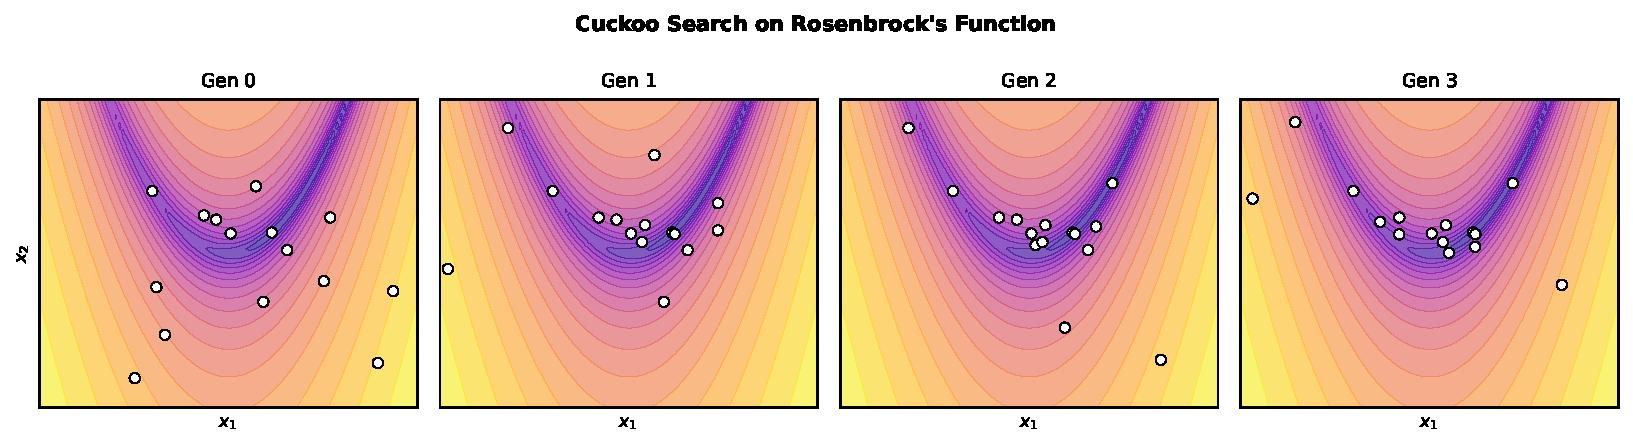
\includegraphics[width=\linewidth]{fig_cuckoo_search.pdf}
      \footnotesize
      Cuckoo search applied to Rosenbrock's function
      $f(\bx) = (1-x_1)^2 + 100(x_2 - x_1^2)^2$, whose global
      minimum is at $(1, 1)$ where $f = 0$.  The nests (white dots)
      gradually concentrate near $(1, 1)$ as the algorithm progresses.
      Rosenbrock's function is notoriously difficult because its
      minimum lies in a narrow, curved valley.
    \end{column}
  \end{columns}

  \begin{alertblock}{Why Cauchy Flights Enable Better Global Exploration}
    A standard Gaussian random walk produces step sizes that are
    almost always small, because the tails of the Gaussian
    distribution decay very rapidly (proportional to $e^{-x^2}$).
    The Cauchy distribution has \emph{heavy tails}: they decay only
    proportionally to $1/x^2$, which is much slower.  This means:
    most iterations, the algorithm makes a small local refinement
    step (the peak of the Cauchy distribution is near zero) ---
    but occasionally it makes a very large jump that can cross an
    entire valley or escape a basin of attraction.  This mix of
    predominantly local steps with rare long-range jumps is
    called a Levy flight pattern and is an efficient strategy for
    complex, multi-modal landscapes.
  \end{alertblock}

\end{frame}

\begin{frame}[fragile]{Cuckoo Search: Python Implementation}
\begin{lstlisting}[style=python, caption={Cuckoo Search with Cauchy flights (Python / NumPy)}]
import numpy as np

def cuckoo_search(f, bounds, pop_size=25, k_max=100,
                  p_a=0.25, m_search_frac=1.0, r=0.01, rng=None):
    rng = rng or np.random.default_rng()
    lo, hi = np.array(bounds).T
    n = len(lo)
    m_search = max(1, int(m_search_frac * pop_size))  # nests that receive a step
    m_abandon = max(1, int(p_a * pop_size))            # nests to abandon each iter

    # Initialise: list of (x, y) pairs sorted by objective value ascending
    pop = [(x, f(x)) for x in rng.uniform(lo, hi, (pop_size, n))]
    pop.sort(key=lambda t: t[1])

    for _ in range(k_max):
        # Step 1: Levy (Cauchy) flight for m_search nests
        for i in range(m_search):
            j = rng.integers(pop_size)                        # pick random nest
            step = rng.standard_cauchy(n) * r * (hi - lo)    # Cauchy step scaled by range
            x_new = np.clip(pop[j][0] + step, lo, hi)
            y_new = f(x_new)
            if y_new < pop[i][1]:                             # greedy acceptance
                pop[i] = (x_new, y_new)
        # Step 2: Sort and abandon the m_abandon worst nests
        pop.sort(key=lambda t: t[1])
        for i in range(pop_size - m_abandon, pop_size):
            x_new = rng.uniform(lo, hi, n)                    # random replacement
            pop[i] = (x_new, f(x_new))
        pop.sort(key=lambda t: t[1])                          # re-sort after abandonment

    return pop[0][0]   # return best nest position (first after sorting)

# Example: Rosenbrock minimum at (1, 1)
f = lambda x: (1 - x[0])**2 + 100*(x[1] - x[0]**2)**2
print(cuckoo_search(f, [(-2, 2), (-1, 3)]))
\end{lstlisting}

  The population is stored as a list of \texttt{(position, objective)}
  tuples, always kept sorted in ascending order of objective value
  (so \texttt{pop[0]} is always the best nest).  The Cauchy step
  \texttt{rng.standard\_cauchy(n) * r * (hi - lo)} scales the
  Cauchy random numbers by $r$ and by the range $(hi - lo)$ so
  that the step size is appropriate for the problem's bounds
  regardless of the actual scale of the design variables.

\end{frame}

\begin{frame}[allowframebreaks]{Cuckoo Search: Key Properties and Parameter Summary}

  \begin{columns}[T]
    \begin{column}{0.52\textwidth}
      \begin{block}{Cauchy vs.\ Gaussian Flights: A Comparison}
        The Cauchy distribution (used to approximate Levy flights)
        has the following properties relevant to optimization:
        \begin{itemize}
          \item Its probability density function has \emph{heavier
                tails} than the Gaussian (normal) distribution.
                Where a Gaussian step of size $10\sigma$ is
                astronomically unlikely (probability $\sim 10^{-23}$),
                a Cauchy step of the same size is merely uncommon
                (probability $\sim 1/100$).
          \item Most Cauchy-distributed steps are small (the peak
                of the distribution is at zero), providing local
                refinement in most iterations.
          \item Occasionally, a very large step occurs --- a
                ``Levy jump'' --- which can move the algorithm
                across a large basin to explore a completely
                different region.  This is the key difference
                from Gaussian random walks.
          \item The scale parameter $r$ (r) controls the typical
                step size: smaller $r$ produces finer local steps,
                larger $r$ produces broader exploration jumps.
        \end{itemize}
      \end{block}

      \begin{block}{Nest Abandonment as a Partial Restart}
        Abandoning the worst $\lfloor m \cdot p_a \rfloor$ nests
        each iteration and replacing them with uniform random samples
        is equivalent to periodically restarting the weakest
        individuals from scratch.  This prevents the entire
        population from clustering around a local minimum while
        preserving the best nests (the elite solutions refined
        over many iterations).  It is a simple but effective strategy
        for maintaining population diversity throughout the search.

        For example, with $m = 25$ and $p_a = 0.25$, we abandon
        $\lfloor 25 \times 0.25 \rfloor = 6$ nests per iteration
        and replace them with random candidates, while keeping the
        top 19 nests intact.
      \end{block}
    \end{column}
    \begin{column}{0.46\textwidth}
      \begin{block}{Computational Complexity}
        \begin{tabular}{ll}
          \toprule
          Step & Cost per iteration \\
          \midrule
          $m_s$ Levy flights & $O(m_s \cdot T_f)$ \\
          Sort nests & $O(m \log m)$ \\
          Abandon and replace $m_a$ nests & $O(m_a \cdot T_f)$ \\
          \midrule
          \textbf{Total per iteration} & $O(m \cdot T_f)$ \\
          \bottomrule
        \end{tabular}
        \vspace{4pt}
        The overall cost is linear in population size $m$ --- the
        same order as PSO and DE, and much cheaper than the firefly
        algorithm's $O(m^2 T_f)$ (m squared times T sub f).
      \end{block}

      \begin{block}{Parameter Summary and Typical Values}
        \begin{tabular}{lll}
          \toprule
          Parameter & Meaning & Typical value \\
          \midrule
          $m$ & population size & 15--50 \\
          $p_a$ & abandonment rate & 0.25 \\
          $r$ & Cauchy scale & 0.01 \\
          $m_s/m$ & search fraction & 1.0 (all nests) \\
          \bottomrule
        \end{tabular}
        \vspace{4pt}
        The abandonment rate $p_a = 0.25$ (25\%) has been found
        to work well across many benchmark problems.  Increasing
        $p_a$ above 0.5 destroys too much progress; decreasing
        it below 0.1 allows poor nests to persist too long.
      \end{block}

      \begin{alertblock}{Key Takeaway}
        Cuckoo search is particularly effective for rugged,
        multi-modal landscapes where occasional large jumps are
        needed to escape basins of attraction.  Its combination of
        heavy-tailed exploration (Cauchy flights) with elite
        preservation (keeping the best nests) makes it robust to
        premature convergence.  The two-mechanism structure ---
        local refinement via flights, diversity via abandonment ---
        mirrors the hybrid philosophy of Section 9.7.
      \end{alertblock}
    \end{column}
  \end{columns}

\end{frame}

% ---------------------------------------------------------------
\section{Hybrid Methods}
% ---------------------------------------------------------------

\begin{frame}[allowframebreaks]{9.7 Hybrid Methods: Combining Global and Local Search}

  Population methods are excellent at \emph{global exploration}: they
  maintain diversity across the design space and can locate the basin
  of attraction of the global minimum even in highly multi-modal
  landscapes.  However, they are often \emph{slow at refining} a
  solution once they are near a minimum --- they approach the optimum
  gradually over many generations, whereas a dedicated local search
  method (such as gradient descent or Nelder-Mead) would converge
  precisely in far fewer evaluations.

  Local search methods (gradient descent, Nelder-Mead simplex, etc.)
  are the opposite: they converge quickly to a precise local minimum
  near their starting point, but they have no mechanism for escaping
  local minima if they start far from the global optimum.

  \textbf{Hybrid methods} combine both strategies: use a population
  method for global exploration to locate promising basins, and
  a local search method for local refinement to exploit those basins
  efficiently.  The key design question is: should the local search
  move the individual to its local minimum (updating its position),
  or should it only be used to compute a better fitness value for
  selection purposes while the individual stays at its original
  position?

  \begin{columns}[T]
    \begin{column}{0.55\textwidth}
      \begin{block}{Philosophy 1: Lamarckian Learning}
        Named after the French biologist Jean-Baptiste Lamarck (1744--1829),
        who proposed that organisms can pass on traits acquired during
        their lifetime directly to their offspring.  In optimization:
        run local search starting from each individual $\bx^{(i)}$
        and \emph{physically move} the individual to the local minimum
        $\bx^{(i)}_{\text{local}}$ found.  The individual's position
        in the population is permanently updated to the refined value.

        \textit{Advantage}: Very fast local refinement.  The population
        quickly fills with locally optimal solutions, and the best
        individual improves dramatically in just a few local-search
        steps.

        \textit{Disadvantage}: The population can prematurely cluster
        around a single local minimum, especially if all individuals
        start in the same basin.  Once moved to their local minima,
        individuals lose their spatial diversity and the ability to
        explore other basins.
      \end{block}

      \begin{block}{Philosophy 2: Baldwinian Learning}
        Named after James Mark Baldwin (1861--1934), who proposed that
        the ability to learn during a lifetime can influence
        evolutionary selection without directly modifying the genome.
        In optimization: run local search from each individual
        $\bx^{(i)}$ to obtain an improved value
        $f(\bx^{(i)}_{\text{local}})$, but use this improved value
        \emph{only for the selection step} (deciding who becomes a
        parent) --- the individual's actual position remains at
        $\bx^{(i)}$.

        \textit{Advantage}: Selection is guided by local-search quality
        without losing population diversity.  Individuals remain
        distributed across different basins, maintaining the ability
        to recombine information from different regions.

        \textit{Disadvantage}: Slower convergence than Lamarckian,
        because the physical positions are not moved to the improved
        locations.  More function evaluations are needed for the same
        final solution quality.
      \end{block}
    \end{column}
    \begin{column}{0.43\textwidth}
      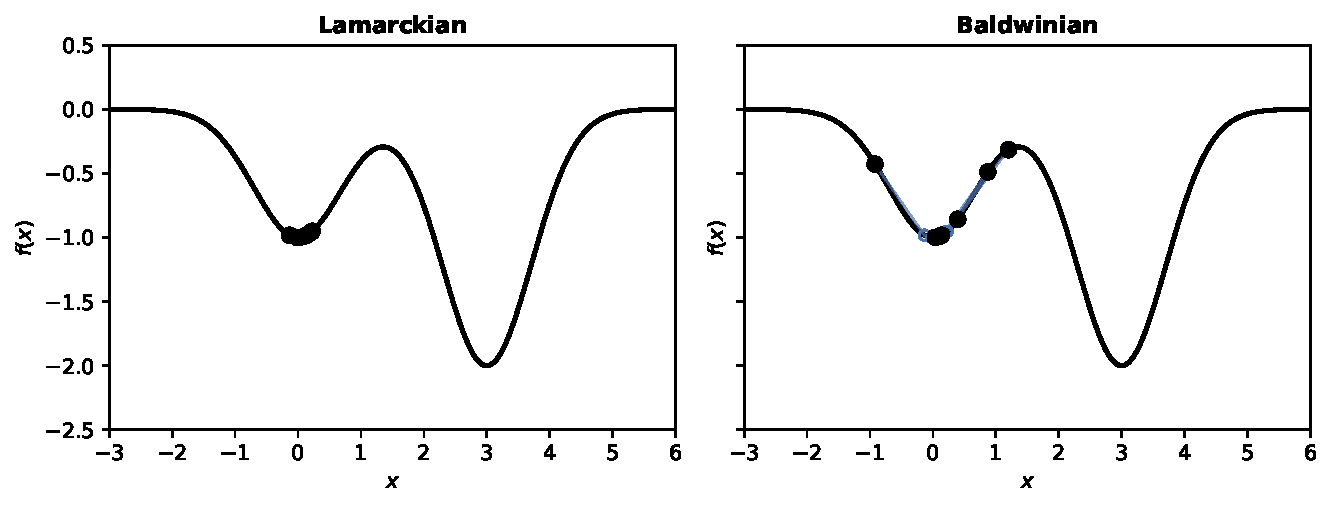
\includegraphics[width=\linewidth]{fig_hybrid_methods.pdf}
      \footnotesize
      Illustration with $f(x) = -e^{-x^2} - 2e^{-(x-3)^2}$
      (two local minima: a shallower one near $x=0$ where $f \approx -1$
      and the global minimum near $x=3$ where $f \approx -2$).

      \textbf{Left (Lamarckian):} all individuals near $x=0$ move
      physically to the local minimum at $x \approx 0$ and cluster
      there --- the global minimum near $x=3$ is missed entirely.

      \textbf{Right (Baldwinian):} individuals stay at their
      original positions (filled dots); local-search evaluations
      (open circles with arrows) inform selection without
      moving the individuals, preserving diversity so crossover
      can still produce offspring near $x=3$.
    \end{column}
  \end{columns}

  \begin{alertblock}{Key Takeaway: When to Use Each Philosophy}
    If the problem has few local minima and you need fast precise
    convergence, Lamarckian learning is effective and straightforward.
    If the landscape is complex with many local minima and you are
    unsure whether the current population is near the global optimum,
    use Baldwinian learning to preserve the population's ability to
    explore multiple basins simultaneously.  As a general rule of
    thumb: when in doubt, use Baldwinian --- it costs no more than
    Lamarckian and is safer on complex landscapes.
  \end{alertblock}

\end{frame}

\begin{frame}[fragile]{Baldwinian Hybrid GA: Python Example}
\begin{lstlisting}[style=python, caption={Baldwinian hybrid GA with local refinement (Python / SciPy)}]
import numpy as np
from scipy.optimize import minimize

def baldwinian_ga(f, bounds, pop_size=30, k_max=50,
                  k_trunc=8, sigma=0.3, rng=None):
    rng = rng or np.random.default_rng()
    lo, hi = np.array(bounds).T
    n = len(lo)
    pop = rng.uniform(lo, hi, (pop_size, n))

    for _ in range(k_max):
        # Baldwinian: use local-search VALUE for selection, keep original POSITION
        def local_val(x):
            res = minimize(f, x, method='Nelder-Mead',
                           options={'maxiter': 20, 'xatol': 1e-4})
            return res.fun   # return improved objective value, NOT the improved position

        y = np.array([local_val(x) for x in pop])   # pop positions are unchanged

        # Standard GA: truncation selection + single-point crossover + Gaussian mutation
        parents = pop[np.argsort(y)[:k_trunc]]
        new_pop = []
        while len(new_pop) < pop_size:
            a, b = parents[rng.choice(k_trunc, 2, replace=False)]
            cp = rng.integers(1, n)
            child = np.concatenate([a[:cp], b[cp:]])
            child += rng.normal(0, sigma, n) * (rng.random(n) < 1/n)
            child = np.clip(child, lo, hi)
            new_pop.append(child)
        pop = np.array(new_pop)   # positions updated by GA crossover/mutation, NOT by local search

    y = np.array([f(x) for x in pop])
    return pop[np.argmin(y)]
\end{lstlisting}

  The critical line is \texttt{return res.fun} instead of
  \texttt{return res.x}.  By returning the improved \emph{objective
  value} (not the improved \emph{position}), we use local search
  only to evaluate the ``potential'' of each individual, keeping
  the population's spatial diversity intact.  The GA then performs
  selection on these local-search-informed fitness scores, so
  individuals near good basins are more likely to become parents,
  even though their positions are not physically moved to the local
  minima.

\end{frame}

\begin{frame}[allowframebreaks]{Lamarckian vs.\ Baldwinian: Worked Example and Comparison}

  \begin{columns}[T]
    \begin{column}{0.50\textwidth}
      \begin{exampleblock}{Worked Example: A Two-Basin Landscape}
        Consider the one-dimensional function:
        \[
          f(x) = -e^{-x^2} - 2e^{-(x-3)^2}
        \]
        where $e$ (Euler's number, approximately 2.718) is the base
        of the natural exponential function.  This function has
        \emph{two local minima}: a shallower one near $x = 0$
        (where $f(0) = -1$) and the global minimum near $x = 3$
        (where $f(3) \approx -2$, meaning it is twice as deep as
        the local minimum).

        Suppose we start with a population of 10 individuals, all
        clustered near $x = 0$.

        \textbf{Under Lamarckian learning:} each individual near
        $x = 0$ is moved by local search to the local minimum at
        $x \approx 0$.  All 10 individuals now sit at the local
        minimum.  All future crossover between these identical
        individuals produces offspring also near $x = 0$.  The
        probability of discovering the global minimum at $x \approx
        3$ becomes essentially zero --- the algorithm is permanently
        trapped.

        \textbf{Under Baldwinian learning:} the selection step
        uses the local-search-improved values (approximately $-1$
        for all individuals near $x = 0$), but the individuals
        remain spread in a small region around $x = 0$.  Gaussian
        mutation can still produce offspring that drift toward $x =
        1, 2,$ or $3$, where local search reveals a fitness of
        approximately $-2$ --- much better than $-1$.  These drifted
        individuals are strongly selected as parents, and the
        population gradually shifts toward the global minimum at
        $x = 3$.
      \end{exampleblock}
    \end{column}
    \begin{column}{0.48\textwidth}
      \begin{block}{Comparison Table}
        \footnotesize
        \begin{tabular}{lll}
          \toprule
          Property & Lamarckian & Baldwinian \\
          \midrule
          Exploits local info & Strongly & Via selection only \\
          Preserves diversity & No & Yes \\
          Convergence speed & Fast locally & Moderate \\
          Global reach & Low (gets trapped) & Higher \\
          Extra cost per gen. & $O(T_\text{local})$ & $O(T_\text{local})$ \\
          Risk of local trap & High & Low \\
          \bottomrule
        \end{tabular}

        \vspace{6pt}
        In this table, $T_\text{local}$ (T sub local) is the cost
        of running the local optimizer on one individual.  With
        Nelder-Mead limited to 20 iterations, $T_\text{local}$ is
        approximately 20 times the cost of a single objective
        evaluation.  Both methods pay this same overhead, but
        Baldwinian uses it more wisely.
      \end{block}

      \vspace{4pt}
      Both methods incur the same additional cost per individual
      per generation: running a local optimizer that performs
      $T_\text{local}$ evaluations.  Since Nelder-Mead or a few
      gradient steps are typically much cheaper than solving the
      original problem, this overhead is usually acceptable and
      pays for itself many times over in improved solution quality.

      \begin{alertblock}{Recommendation}
        In practice, Baldwinian learning is the recommended default
        for hybrid methods.  It consistently outperforms Lamarckian
        on problems with multiple local minima, at essentially the
        same computational cost, because it never sacrifices
        diversity for local precision.
      \end{alertblock}
    \end{column}
  \end{columns}

\end{frame}

% ---------------------------------------------------------------
\section{Summary \& Exercises}
% ---------------------------------------------------------------

\begin{frame}[allowframebreaks]{Chapter 9 Summary}

  This chapter introduced the family of \emph{population methods}
  for optimization --- algorithms that maintain a collection of
  $m$ (m) candidate solutions (a ``population'') and evolve them
  collectively over many iterations called generations.  Unlike
  single-point methods (gradient descent, Nelder-Mead), population
  methods share information across the design space, making them
  much more robust to local minima on complex, multi-modal objectives.

  \begin{columns}[T]
    \begin{column}{0.50\textwidth}
      \begin{block}{Genetic Algorithms (Section 9.2)}
        GAs are biologically inspired.  Three operators are applied
        each generation: (1) \textbf{Selection} converts objectives
        to fitness scores and biases reproduction toward better
        individuals.  (2) \textbf{Crossover} combines gene sequences
        from two parents to create offspring, mixing good gene
        combinations from different individuals.  (3) \textbf{Mutation}
        introduces random perturbations so that new gene values can
        be discovered beyond those present in the initial population.
        GAs work naturally on both discrete (binary, integer) and
        continuous design spaces.
      \end{block}

      \begin{block}{Differential Evolution (Section 9.3)}
        DE uses the difference vector between two randomly chosen
        population members as a self-adapting perturbation.  The
        perturbation magnitude automatically scales with population
        diversity: large early (exploration) and small later
        (refinement).  Greedy acceptance ensures the population never
        degrades.  DE is among the most effective methods for
        continuous, multi-modal problems and requires only two
        parameters ($p$ and $w$).
      \end{block}

      \begin{block}{Particle Swarm Optimization (Section 9.4)}
        PSO equips each particle with a velocity that combines
        three forces: inertia (keep moving in the current direction),
        cognitive pull (move toward personal best), and social pull
        (move toward global best).  PSO is fast, easy to implement,
        and has few parameters.  It is often the best first method
        to try on a new continuous optimization problem.
      \end{block}
    \end{column}
    \begin{column}{0.48\textwidth}
      \begin{block}{Firefly Algorithm (Section 9.5)}
        The firefly algorithm models pairwise attraction based on
        brightness (fitness): dimmer individuals move toward brighter
        ones with attraction strength $\beta(r) = \beta_0 e^{-\gamma
        r^2}$ (beta-zero times e to the minus gamma r squared)
        that decays exponentially with distance $r$ (r), creating
        natural local clustering.  Main limitation: $O(m^2)$ cost
        per iteration.
      \end{block}

      \begin{block}{Cuckoo Search (Section 9.6)}
        Cuckoo search uses heavy-tailed Cauchy (Levy) flights for
        exploration, enabling occasional large jumps that escape
        local minima.  Nest abandonment (discarding and randomly
        replacing the worst $p_a$ (p sub a) fraction of solutions)
        acts as a partial restart maintaining diversity.  Overall
        cost is $O(m \cdot T_f)$ per iteration --- linear in
        population size, like PSO and DE.
      \end{block}

      \begin{block}{Hybrid Methods (Section 9.7)}
        Any population method can be enhanced by embedding a local
        search step each generation.  \textbf{Lamarckian learning}
        moves individuals physically to their local minima (fast but
        loses diversity; may trap the population at a local minimum).
        \textbf{Baldwinian learning} uses local-search values only
        for selection, keeping individuals at their original positions
        (preserves diversity and global reach at the same cost per
        generation).  Baldwinian is the recommended default.
      \end{block}
    \end{column}
  \end{columns}

\end{frame}

\begin{frame}[allowframebreaks]{Method Comparison: Complexity and Practical Guidance}

  \begin{block}{Algorithm Complexity and Parameter Summary}
    \footnotesize
    \begin{tabular}{lllll}
      \toprule
      Method & Per-iteration cost & Key parameters & Strengths & Best for \\
      \midrule
      Genetic Algorithm
        & $O(m(T_f + n\log m))$
        & $m$, $k$, $\lambda$, $\sigma$
        & Flexible encoding
        & Discrete + continuous \\
      Differential Evolution
        & $O(m \cdot T_f)$
        & $m$, $p$, $w$
        & Self-adapting step size
        & Continuous, multi-modal \\
      PSO
        & $O(m \cdot T_f)$
        & $m$, $w$, $c_1$, $c_2$
        & Fast, simple
        & Continuous, fast conv. \\
      Firefly
        & $O(m^2 T_f)$
        & $m$, $\alpha$, $\beta_0$, $\gamma$
        & Pairwise attraction
        & Multi-modal, small $m$ \\
      Cuckoo Search
        & $O(m \cdot T_f)$
        & $m$, $p_a$, $r$
        & Long-range jumps
        & Rugged, continuous \\
      \bottomrule
    \end{tabular}
    \vspace{4pt}
    In this table: $m$ (m) is population size, $T_f$ (T sub f) is
    cost of one objective evaluation, $n$ (n) is number of design
    variables, $\lambda$ (lambda) is mutation rate, $\sigma$ (sigma)
    is mutation standard deviation, $w$ (w) is differential weight
    or inertia, $c_1$ (c sub 1) is cognitive coefficient,
    $c_2$ (c sub 2) is social coefficient, $\alpha$ (alpha) is
    random walk step, $\beta_0$ (beta sub 0) is max attractiveness,
    $\gamma$ (gamma) is light absorption, $p_a$ (p sub a) is
    abandonment probability, $r$ (r) is Cauchy scale.
  \end{block}

  \framebreak

  \begin{block}{Practical Guidance: Which Method to Use?}
    \textbf{Unknown landscape --- first attempt.}
    Start with PSO or DE.  Both have linear cost in $m$, few
    parameters, and are robust across a wide range of continuous
    problems.  PSO is particularly easy to tune (adjust $w$ to
    control exploration vs.\ exploitation).

    \textbf{Mixed-integer or combinatorial problem.}
    Use a GA with an appropriate encoding: binary genes with
    bit-flip mutation for combinatorial problems, or real-valued
    genes with Gaussian mutation for continuous variables.

    \textbf{Highly multi-modal landscape.}
    Cuckoo search (Levy flights enable long-range jumps across
    basins) or the firefly algorithm (pairwise attraction can
    maintain multiple sub-populations around different modes
    simultaneously) are good choices.

    \textbf{Need fast local refinement after global search.}
    Wrap any population method with Baldwinian (preferred) or
    Lamarckian local search.  Use a lightweight local optimizer
    such as Nelder-Mead (derivative-free) or L-BFGS (gradient-based
    if derivatives are available).

    \textbf{Limited evaluation budget (expensive $f$).}
    Population size $m$ is the primary lever: a smaller $m$ uses
    fewer evaluations per generation but may miss the global
    optimum.  With a budget of $B$ total evaluations, set $m$
    and $k_{\max}$ so that $m \times k_{\max} = B$.  Larger $m$
    with fewer generations favours exploration; smaller $m$ with
    more generations favours exploitation.
  \end{block}

\end{frame}

\begin{frame}[allowframebreaks]{Selected Exercises with Worked Solutions}

  \begin{enumerate}
    \item[\textbf{9.1}] \textit{What is the purpose of the selection
      operation in genetic algorithms?}

      \textbf{Solution.}  Selection serves to bias reproductive
      success toward individuals with lower objective values (higher
      fitness), ensuring that the gene pool of the next generation
      is dominated by better-performing individuals.  Without
      selection, the GA would perform random crossover and mutation
      with no pressure toward improvement --- it would behave like
      a random search.  Selection is the mechanism by which useful
      genetic ``building blocks'' (combinations of gene values that
      contribute to low objective values) are preserved and amplified
      across generations.  Without selection, good gene combinations
      appear randomly by chance just as often as bad ones, and the
      population does not converge.

    \item[\textbf{9.2}] \textit{Why does mutation play a fundamental
      role in GAs? If you suspect there is a better optimum
      elsewhere, how should you adjust $\lambda$ (lambda)?}

      \textbf{Solution.}  Mutation is fundamental because crossover
      alone can only combine gene values that already exist in the
      population.  If the optimal solution requires a gene value
      that was not present in any individual at initialisation ---
      for example, if the global optimum requires $x_1 = 7.3$ but
      all initial individuals have $x_1 \in [-5, 0]$ --- crossover
      can \emph{never} discover it.  Mutation introduces new gene
      values by random perturbation (adding $\varepsilon \sim
      \mathcal{N}(0, \sigma^2)$), enabling the GA to explore regions
      not represented in the initial population.

      If a better optimum is suspected elsewhere (for example, the
      best individual has not improved for many consecutive
      generations), \emph{increase} $\lambda$ above the default
      $1/n$ --- for example, to $3/n$ or $5/n$ --- to generate
      more exploration per generation at the cost of potentially
      disrupting near-optimal solutions.

    \item[\textbf{9.3}] \textit{PSO converges to a non-global
      minimum. How can you adjust the parameters?}

      \textbf{Solution.}  Premature convergence in PSO usually means
      the social force $c_2 r_2 (\bx^* - \bx)$ is overwhelming all
      particles toward the current global best, which happens to be
      a local (not global) minimum.  Three remedies:
      (1) Increase the number of particles $n_{\text{particles}}$
      so the initial population is more spread out and more likely
      to have at least one particle near the true global minimum.
      (2) Increase the cognitive coefficient $c_1$ relative to $c_2$,
      strengthening each particle's attraction to its own personal
      best (individual memory) and weakening the social pull.
      (3) Increase the inertia weight $w$ to give particles more
      momentum to overshoot the local attractor and explore beyond
      it.  If the problem is high-dimensional, consider running
      multiple independent PSO instances (multi-start).

    \item[\textbf{9.4}] \textit{Compare five DE variants on Ackley's
      function and explain the results.}

      \textbf{Solution.}
      (1) $w = 0$: worst --- the trial vector $\mathbf{z} = \ba +
      0 \cdot (\bb - \bc) = \ba$ contains only existing population
      values; no new gene values outside the current range can be
      generated; the algorithm immediately stagnates.
      (2) $\ba = \bx^{(i)}$ (DE/current): biased toward local
      exploration around each individual, hard to escape local
      minima on highly multi-modal Ackley's function.
      (3) Standard $p = 0.5, w = 0.5$: balanced --- a good default
      that performs reasonably on most problems.
      (4) $p = 0.9$: high crossover probability means nearly every
      dimension is replaced by the trial vector; performs almost as
      well as $p = 1.0$.
      (5) $p = 1.0$ (guaranteed crossover): best performer on
      Ackley's function --- every dimension is updated at every
      iteration, maximising information flow from the self-adapting
      differential perturbation.
  \end{enumerate}

\end{frame}

% ---------------------------------------------------------------
\begin{frame}[allowframebreaks]{References}
  \begin{itemize}
    \item M.\ J.\ Kochenderfer \& T.\ A.\ Wheeler,
          \textit{Algorithms for Optimization}, 2nd ed., MIT Press, 2026.
          Chapter 9: Population Methods.
    \item J.\ H.\ Holland, \textit{Adaptation in Natural and Artificial
          Systems}, MIT Press, 1992.  (Original treatment of
          Genetic Algorithms and the schema theorem.)
    \item R.\ Storn \& K.\ Price, ``Differential Evolution --- a simple
          and efficient heuristic for global optimization over
          continuous spaces,'' \textit{Journal of Global Optimization},
          11(4):341--359, 1997.
    \item J.\ Kennedy \& R.\ Eberhart, ``Particle Swarm Optimization,''
          \textit{Proceedings of IEEE International Conference on
          Neural Networks (ICNN)}, pp.\ 1942--1948, 1995.
    \item X.-S.\ Yang, ``Firefly Algorithms for Multimodal
          Optimization,'' in \textit{Stochastic Algorithms:
          Foundations and Applications (SAGA)}, Lecture Notes in
          Computer Science, vol.\ 5792, Springer, 2009.
    \item X.-S.\ Yang \& S.\ Deb, ``Cuckoo Search via Levy Flights,''
          in \textit{Proceedings of the World Congress on Nature \&
          Biologically Inspired Computing (NaBIC)}, pp.\ 210--214,
          IEEE Press, 2009.
  \end{itemize}
\end{frame}

% ---------------------------------------------------------------
\end{document}
